% A Mathematical Study of COVID-19 Using a SEIQR Epidemic Model (LaTeX source)
% Compile with pdfLaTeX, run twice so the table of contents and citations are filled in.
% Needs the folders charts/ (Fig01-Fig25 PNG) and logos/ next to this file.
\documentclass[12pt,a4paper]{article}
\usepackage[utf8]{inputenc}
\usepackage[T1]{fontenc}
\usepackage{mathptmx}
\usepackage[a4paper,margin=2.54cm]{geometry}
\usepackage{amsmath,amssymb,amsthm}
\usepackage{graphicx}
\usepackage{float}
\usepackage{longtable,array,colortbl}
\usepackage[table]{xcolor}
\usepackage{setspace}
\usepackage{titlesec}
\usepackage{enumitem}
\usepackage{listings}
\usepackage[labelfont=bf,font=small]{caption}
\usepackage{url}
\usepackage[colorlinks=true,linkcolor=blue!40!black,citecolor=blue!40!black,urlcolor=blue!40!black,pdfencoding=auto,unicode]{hyperref}
\definecolor{dblue}{HTML}{1F3864}
\definecolor{mblue}{HTML}{2F5496}
\titleformat{\section}{\Large\bfseries\color{dblue}}{\thesection.}{0.6em}{}
\titleformat{\subsection}{\large\bfseries\color{mblue}}{\thesubsection}{0.6em}{}
\titleformat{\subsubsection}{\normalsize\bfseries\itshape\color{mblue}}{}{0em}{}
\setcounter{secnumdepth}{2}
\setcounter{tocdepth}{3}
\onehalfspacing
\renewcommand{\contentsname}{Table of Contents}
\setlength{\parindent}{0pt}
\setlength{\parskip}{6pt}
\newtheorem{theorem}{Theorem}
\theoremstyle{definition}
\lstset{basicstyle=\ttfamily\footnotesize,breaklines=true,breakatwhitespace=false,frame=single,backgroundcolor=\color{black!4},columns=fullflexible,keepspaces=true,showstringspaces=false,commentstyle=\color{green!40!black},keywordstyle=\color{blue!60!black},xleftmargin=0pt}
\renewcommand{\arraystretch}{1.25}
\setlength{\LTpre}{6pt}\setlength{\LTpost}{6pt}
\hypersetup{pdftitle={A Mathematical Study of COVID-19 Using a SEIQR Epidemic Model},pdfauthor={Shrestha Sarkar}}
\begin{document}
\pagenumbering{gobble}
\begin{titlepage}
\centering
\vspace*{1.5cm}
{\LARGE\bfseries\color{dblue} A Mathematical Study of COVID-19\\[4pt] Using a SEIQR Epidemic Model\par}
\vspace{0.6cm}
{\itshape B.Sc.\ (Hons.) Mathematics -- Final Semester Project (January--March 2022)\par}
\vspace{1.5cm}
{\Large\bfseries Asansol Girls' College\par}
\vspace{4pt}
{\Large\bfseries Kazi Nazrul University\par}
\vspace{1cm}
\includegraphics[height=3.2cm]{logos/college.png}\hspace{2.5cm}\includegraphics[height=3.2cm]{logos/university.png}
\vfill
\raggedright
\begin{tabular}{@{}p{0.42\textwidth}p{0.5\textwidth}@{}}
\textbf{Submitted by:} & \textbf{Submitted to:}\\
Shrestha Sarkar & Dr.\ Fahad Al Basir (HOD)\\
{\small Registration No.: KNU19101001668} & Assistant Prof.\ Chandan Kumar Adhak
\end{tabular}
\vspace{2cm}
\end{titlepage}
\clearpage
\pagenumbering{roman}
\section*{Certificate}
\addcontentsline{toc}{section}{Certificate}
This is to certify that the project report entitled “A Mathematical Study of COVID-19 Using a SEIQR Epidemic Model”, submitted by Shrestha Sarkar (Registration No. KNU19101001668), a student of B.Sc. (Hons.) Mathematics (Semester VI) at Asansol Girls' College, affiliated to Kazi Nazrul University, is a record of bona fide work carried out by her under our guidance and supervision, in partial fulfilment of the requirements for the degree of Bachelor of Science (Honours) in Mathematics.

To the best of our knowledge, the work has not been submitted to any other university or institution for the award of any degree or diploma.

We wish her every success in her future endeavours.

\vspace{1em}
Date: \underline{\hspace{4cm}}\\[2pt]
Place: Asansol

\vspace{2.5cm}
\noindent
\begin{tabular}{@{}p{0.48\textwidth}p{0.48\textwidth}@{}}
\rule{6cm}{0.4pt} & \rule{6cm}{0.4pt}\\
\textbf{Dr.\ Fahad Al Basir} & \textbf{Chandan Kumar Adhak}\\
Head of the Department & Assistant Professor\\
Department of Mathematics & Department of Mathematics\\
Asansol Girls' College & Asansol Girls' College
\end{tabular}
\clearpage
\section*{Declaration}
\addcontentsline{toc}{section}{Declaration}
I, Shrestha Sarkar, Registration No. KNU19101001668, a student of B.Sc. (Hons.) Mathematics (Semester VI) at Asansol Girls' College, Kazi Nazrul University, hereby declare that the project report entitled “A Mathematical Study of COVID-19 Using a SEIQR Epidemic Model” is my own work, carried out under the guidance of Dr. Fahad Al Basir (Head of the Department) and Assistant Professor Chandan Kumar Adhak.

To the best of my knowledge, this work has not been submitted previously to any other university or institution for the award of any degree or diploma. All sources of information used in this report have been acknowledged in the references.

\vspace{1.5em}
\textbf{Date: 25/03/2022}\\[2pt]
Place: Asansol

\vspace{1.5cm}
\hfill\begin{minipage}{0.5\textwidth}
\raggedleft
\rule{6cm}{0.4pt}\\
\textbf{Shrestha Sarkar}\\
Registration No.: KNU19101001668\\
B.Sc.\ (Hons.) Mathematics, Semester VI
\end{minipage}
\clearpage
\section*{Acknowledgement}
\addcontentsline{toc}{section}{Acknowledgement}
I would like to express my sincere gratitude to my project supervisors, Dr. Fahad Al Basir, Head of the Department of Mathematics, and Assistant Professor Chandan Kumar Adhak, for their guidance, encouragement and valuable suggestions throughout this project.

I am also thankful to all the faculty members of the Department of Mathematics, Asansol Girls' College, and to Kazi Nazrul University for giving me the opportunity to carry out this work.

I thank the authors of the books and papers listed in the references, especially N. Bairagi's Introductory Mathematical Biology, which helped me to understand the model.

Finally, I thank my family and friends for their constant support and encouragement.

\vspace{1.5em}
\hfill\begin{minipage}{0.5\textwidth}
\raggedleft
\textbf{Shrestha Sarkar}\\
Registration No.: KNU19101001668
\end{minipage}
\clearpage

\tableofcontents
\clearpage
\pagenumbering{arabic}

\section*{Abstract}
\addcontentsline{toc}{section}{Abstract}

This project studies the spread and control of COVID-19 with a deterministic compartmental model having five classes: Susceptible $(S)$, Exposed $(E)$, Infected $(I)$, Isolated $(Q)$ and Recovered $(R)$. The basic reproduction number $R_{0}$ is obtained by the next-generation matrix method and acts as a threshold. When $R_{0} < 1$ the disease-free equilibrium is locally asymptotically stable and the infection dies out. When $R_{0} > 1$ the disease-free equilibrium is unstable and a unique endemic equilibrium, which is locally asymptotically stable, appears. Numerical simulations for $R_{0} = 2.35$ and $R_{0} = 0.59$ illustrate the two behaviours, and a sensitivity analysis shows how faster isolation of exposed and infected people lowers $R_{0}$. The parameters are compared with published estimates, the influence of each parameter on $R_{0}$ is quantified, and a lockdown scenario shows that its timing and duration decide whether the epidemic is suppressed or only delayed. An extended model with disease death and vaccination is analysed, and Euler's method is compared with the fourth-order Runge–Kutta method.


\section{Introduction}

Mathematical models help us understand how an infection behaves when it enters a community and under which conditions it will be wiped out or will continue \cite{r1,r3,r4}. COVID-19 became a major concern for researchers, governments and the public because of its high rate of spread and the large number of deaths it caused \cite{r8}. The disease is caused by a newly discovered coronavirus, SARS-CoV-2, first reported in Wuhan, China, in December 2019. It is transmitted mainly through respiratory droplets and smaller aerosol particles released when an infected person coughs, sneezes, talks or exhales.


Before the epidemic, life was normal: schools, colleges, markets and shops were open. Once COVID-19 spread, many of these activities were restricted by the government to slow the infection. Mathematics lets us describe this situation logically: we write equations for how people move between stages of the disease, and then ask under what conditions the virus disappears and under what conditions it persists.


The objectives of this project are:


\begin{itemize}
\item to formulate a SEIQR model that includes an isolation (quarantine) class;
\item to find the equilibria of the model and the basic reproduction number $R_{0}$;
\item to analyse the stability of the equilibria and the role of $R_{0}$ as a threshold;
\item to simulate the model for $R_{0} > 1$ and $R_{0} < 1$;
\item to study how isolation rates change $R_{0}$ and the size of an outbreak;
\item to find which parameters influence $R_{0}$ most and compare parameter values with published estimates; and
\item to study the effect of a lockdown on the epidemic.
\end{itemize}

\section{Model Formulation}

\subsection{Assumptions}

\begin{itemize}
\item The population is homogeneous and mixes uniformly. New infections occur at rate $\beta S(E + I)$ (mass-action incidence).
\item Individuals in $E$ and in $I$ can transmit the virus (pre-symptomatic transmission has been reported for COVID-19). Isolated individuals $(Q)$ do not transmit.
\item An exposed individual either becomes infected (rate $\alpha )$ or is identified and isolated (rate $\gamma )$. Infected individuals are isolated at rate $\sigma$.
\item Isolated individuals recover at rate $\theta$. Recovered individuals stay immune during the study period.
\item New individuals enter $S$ at constant rate A. Natural death occurs at rate $\mu$ in every compartment. In the base model, deaths caused by COVID-19 are not modelled separately; the extended model of Section 15 adds a disease death rate.
\item All parameters are constant in time.
\end{itemize}

\subsection{Variables and parameters}

\begin{longtable}{>{\raggedright\arraybackslash}p{\dimexpr(\linewidth-6\tabcolsep)*1037/9063\relax}>{\raggedright\arraybackslash}p{\dimexpr(\linewidth-6\tabcolsep)*6126/9063\relax}>{\centering\arraybackslash}p{\dimexpr(\linewidth-6\tabcolsep)*1900/9063\relax}}
\hline
\rowcolor[HTML]{D9E2F3}\textbf{Symbol} & \textbf{Meaning} & \textbf{Unit} \\ \hline
\endhead
$S$ & Susceptible individuals & people \\ \hline
$E$ & Exposed: infected but not yet showing symptoms (assumed able to transmit) & people \\ \hline
$I$ & Infected (symptomatic, not yet isolated) & people \\ \hline
$Q$ & Isolated (quarantined); assumed not to transmit & people \\ \hline
$R$ & Recovered & people \\ \hline
A & Recruitment (birth) rate into $S$ & people/day \\ \hline
$\mu$ & Natural death rate (all compartments) & 1/day \\ \hline
$\beta$ & Transmission rate & 1/(person·day) \\ \hline
$\alpha$ & Rate at which exposed people become infected (written $\pi$ in the handwritten notes) & 1/day \\ \hline
$\gamma$ & Rate at which exposed people are isolated (precautions, contact tracing) & 1/day \\ \hline
$\sigma$ & Rate at which infected people are isolated & 1/day \\ \hline
$\theta$ & Rate at which isolated people recover & 1/day \\ \hline
\end{longtable}

\textit{Note: the symbol $\alpha$ replaces $\pi$ used in the handwritten report, to avoid confusion with the number 3.14159\ldots{}}


\subsection{The model equations}

\begin{figure}[H]
\centering
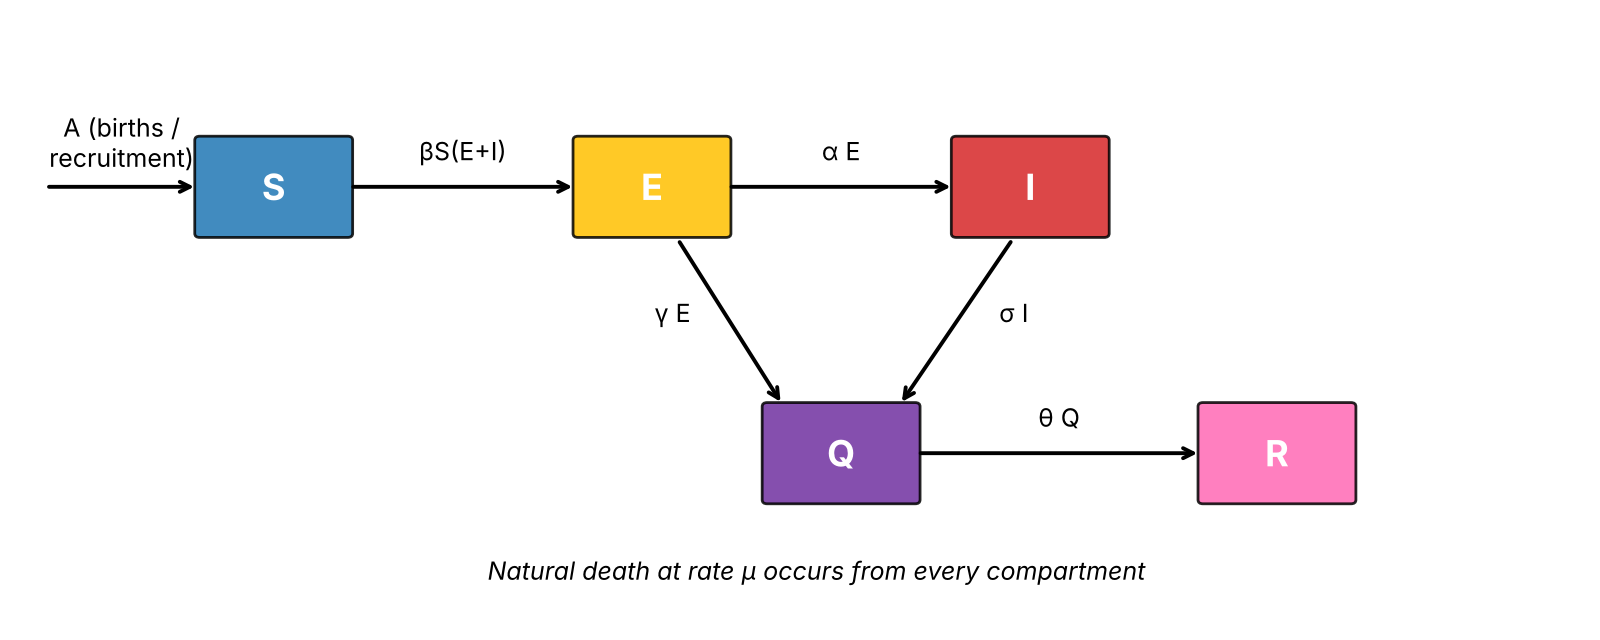
\includegraphics[width=0.9\linewidth]{charts/Fig01_Flow_Diagram.png}
\caption{Flow diagram of the SEIQR model.}
\end{figure}

Following the flow in Figure 1, the model is the system of ordinary differential equations


\begin{equation}
\frac{dS}{dt} = A - \mu S - \beta S(E+I)
\end{equation}

\begin{equation}
\frac{dE}{dt} = \beta S(E+I) - (\alpha+\mu+\gamma)E
\end{equation}

\begin{equation}
\frac{dI}{dt} = \alpha E - (\sigma+\mu)I
\end{equation}

\begin{equation}
\frac{dQ}{dt} = \gamma E + \sigma I - (\theta+\mu)Q
\end{equation}

\begin{equation}
\frac{dR}{dt} = \theta Q - \mu R
\end{equation}

To shorten the algebra we write


\begin{equation}
k_1 = \alpha+\mu+\gamma,\qquad k_2 = \sigma+\mu,\qquad k_3 = \theta+\mu
\end{equation}

\section{Total Population and the Disease-Free Equilibrium}

Let $N = S + E + I + Q + R$. Adding the five equations, all transfer terms cancel and we obtain


\begin{equation}
\frac{dN}{dt} = A - \mu N
\end{equation}

This linear equation has the solution


\begin{equation}
N(t) = \frac{A}{\mu} + \left(N_0 - \frac{A}{\mu}\right)e^{-\mu t}
\end{equation}

so $N(t) \to N^* = A/\mu$ as $t \to \infty$. Setting $E = I = Q = R = 0$ and all derivatives to zero gives the disease-free equilibrium


\begin{equation}
C_0 = \left(\frac{A}{\mu},0,0,0,0\right) = (N^*,0,0,0,0)
\end{equation}

If every compartment is divided by $N^*$, this point is written $C_{0} = (1$, 0, 0, 0, 0), which is the form used in the handwritten report.


\section{Classification of the Model}

The model belongs to mathematical epidemiology, a branch of mathematical biology. Its properties are summarised below.


\begin{longtable}{>{\raggedright\arraybackslash}p{\dimexpr(\linewidth-4\tabcolsep)*2600/9026\relax}>{\raggedright\arraybackslash}p{\dimexpr(\linewidth-4\tabcolsep)*6426/9026\relax}}
\hline
\rowcolor[HTML]{D9E2F3}\textbf{Type} & \textbf{Reason} \\ \hline
\endhead
Epidemiological model & It studies transmission, thresholds $(R_{0})$ and disease-free versus endemic states. \\ \hline
Compartmental (SEIQR) & The population is divided into $S$, $E$, $I$, $Q$ and $R$. \\ \hline
Deterministic & Ordinary differential equations with no random terms. \\ \hline
Nonlinear, coupled & The term $\beta S(E + I)$ multiplies unknown functions. \\ \hline
With demography & Birth (A) and natural death $(\mu )$ are included. \\ \hline
With intervention & The class $Q$ represents isolation measures. \\ \hline
Autonomous, continuous time & No explicit dependence on $t$; time is continuous. \\ \hline
\end{longtable}

In one sentence: the model is a deterministic, nonlinear, compartmental epidemic model with demography and isolation, written as a system of autonomous ordinary differential equations.


\section{Comparison with the SIR and SEIR Models}

In this section only, $\rho$ denotes the recovery rate and $\kappa$ the incubation-to-infectious rate of the classical models. They are not the same as $\gamma$ and $\sigma$ of the SEIQR model.


\subsection{The SIR model}

The SIR model of Kermack and McKendrick \cite{r1} has a closed population with no births or deaths, uniform mixing and permanent immunity:


\begin{equation}
\frac{dS}{dt} = -\beta SI,\qquad \frac{dI}{dt} = \beta SI - \rho I,\qquad \frac{dR}{dt} = \rho I
\end{equation}

The mean infectious period is $1/\rho$. With $S_{0}$ the initial susceptible number, $R_{0} = \beta S_{0}/\rho$ (or $\beta /\rho$ for a normalised population). Near the disease-free state $dI/dt \approx (\beta S_{0} - \rho )I$, so the infection grows if $R_{0} > 1$ and dies out if $R_{0} < 1$; this is the threshold phenomenon. The epidemic peak occurs when $dI/dt = 0$, that is when $S = \rho /\beta$. Dividing the two equations gives an implicit relation


\begin{equation}
I + S - \frac{\rho}{\beta}\ln S = \text{constant}
\end{equation}

which describes the S–I trajectories but does not give $S(t)$ or $I(t)$ explicitly.


\subsection{The SEIR model}

SEIR adds an exposed class for the incubation period:


\begin{equation}
\frac{dS}{dt}=-\beta SI,\quad \frac{dE}{dt}=\beta SI-\kappa E,\quad \frac{dI}{dt}=\kappa E-\rho I,\quad \frac{dR}{dt}=\rho I
\end{equation}

The incubation period is $1/\kappa$. People move $S \to E \to I \to R$, and $R_{0} = \beta S_{0}/\rho$ as before, but the epidemic peak is delayed because of the incubation stage. In the classical SEIR model exposed people are not infectious.


\subsection{Relation to the SEIQR model}

The SEIQR model extends SEIR in four ways: it adds an isolation class $Q$, it includes births and deaths, exposed people are allowed to transmit, and exposed people can be isolated directly (rate $\gamma )$. Because exposed people transmit, the formula for $R_{0}$ below has two terms instead of one.


\section{The Basic Reproduction Number $R_{0}$}

The basic reproduction number $R_{0}$ is the average number of new infections caused by one infected individual placed in a fully susceptible population. It is computed at $C_{0}$ with the next-generation matrix method \cite{r5,r6}. The infected compartments are $(E$, $I)$. Let F be the matrix of new-infection terms and $V$ the matrix of transitions between and out of $E$ and $I$, both evaluated at $C_{0}$ (where $S = N^*)$:


\[
F = \begin{pmatrix}\beta N^* & \beta N^*\\ 0 & 0\end{pmatrix},\qquad V = \begin{pmatrix}k_1 & 0\\ -\alpha & k_2\end{pmatrix},\qquad V^{-1} = \frac{1}{k_1k_2}\begin{pmatrix}k_2 & 0\\ \alpha & k_1\end{pmatrix}
\]

The next-generation matrix is $FV^{-1} = [\beta N^*/(k_{1}k_{2})]$ times the matrix with first row $(k_{2} + \alpha$, $k_{1})$ and second row (0, 0). Its only non-zero eigenvalue is its spectral radius,


\begin{equation}
R_0 = \frac{\beta N^*(k_2+\alpha)}{k_1k_2} = \frac{\beta A}{\mu}\left[\frac{1}{k_1}+\frac{\alpha}{k_1k_2}\right]
\end{equation}

Interpretation: an exposed person transmits for an average time $1/k_{1}$; with probability $\alpha /k_{1}$ he or she becomes infected and then transmits for a further average time $1/k_{2}$. The two terms in the brackets are these two contributions. Note that $\theta$ does not appear in $R_{0}$, because isolated people do not transmit.


\subsection{Numerical example}

The parameter values below are illustrative. They are not estimated from real data. They were chosen so that $R_{0}$ lies on each side of 1, with $R_{0}$ in Case 1 comparable to early estimates for COVID-19.


\begin{longtable}{>{\raggedright\arraybackslash}p{\dimexpr(\linewidth-6\tabcolsep)*3200/9026\relax}>{\raggedright\arraybackslash}p{\dimexpr(\linewidth-6\tabcolsep)*2913/9026\relax}>{\raggedright\arraybackslash}p{\dimexpr(\linewidth-6\tabcolsep)*2913/9026\relax}}
\hline
\rowcolor[HTML]{D9E2F3}\textbf{Quantity} & \textbf{Case 1 $(R_{0} > 1)$} & \textbf{Case 2 $(R_{0} < 1)$} \\ \hline
\endhead
A (people/day) & 100 & 100 \\ \hline
$\mu$ (1/day) & 0.02 & 0.02 \\ \hline
$\beta$ (1/(person·day)) & $4 \times 10^{-5}$ & $1 \times 10^{-5}$ \\ \hline
$\alpha$, $\gamma$, $\sigma$, $\theta$ (1/day) & 0.1, 0.05, 0.08, 0.07 & 0.1, 0.05, 0.08, 0.07 \\ \hline
$N^* = A/\mu$ & 5000 & 5000 \\ \hline
$k_{1}$, $k_{2}$, $k_{3}$ & 0.17, 0.10, 0.09 & 0.17, 0.10, 0.09 \\ \hline
$1/k_{1} + \alpha /(k_{1}k_{2})$ & 5.882 + 5.882 = 11.765 & 11.765 \\ \hline
$R_{0}$ & 0.2 $\times$ 11.765 = 2.353 & 0.05 $\times$ 11.765 = 0.588 \\ \hline
Initial state & $S = 4990$, $E = 10$, $I = Q = R = 0$ & $S = 4990$, $E = 10$, $I = Q = R = 0$ \\ \hline
\end{longtable}

With these values the critical transmission rate $(R_{0} = 1)$ is $\beta = 1/(N^* \times 11.765) \approx 1.7 \times 10^{-5}$. Case 1 is above it and Case 2 is below it.


\subsection{Parameter values and published estimates}

The parameter values of Cases 1 and 2 are illustrative. The table compares them with published estimates for COVID-19.


\begin{longtable}{>{\raggedright\arraybackslash}p{\dimexpr(\linewidth-8\tabcolsep)*1037/9163\relax}>{\raggedright\arraybackslash}p{\dimexpr(\linewidth-8\tabcolsep)*1700/9163\relax}>{\raggedright\arraybackslash}p{\dimexpr(\linewidth-8\tabcolsep)*5326/9163\relax}>{\centering\arraybackslash}p{\dimexpr(\linewidth-8\tabcolsep)*1100/9163\relax}}
\hline
\rowcolor[HTML]{D9E2F3}\textbf{Parameter} & \textbf{Value used} & \textbf{Published estimate} & \textbf{Source} \\ \hline
\endhead
$\beta$ & $4 \times 10^{-5}$ (Case 1), $1 \times 10^{-5}$ (Case 2) & Not measured directly. It is chosen so that $R_{0}$ is realistic: early estimate $R_{0} = 2.2$ (95\% CI 1.4–3.9) & \cite{r10} \\ \hline
$\alpha$ & 0.1 per day & Mean incubation period 5.1 days (95\% CI 4.5–5.8) and 5.2 days (95\% CI 4.1–7.0), so $\alpha \approx 0.19$ per day & \cite{r9}, \cite{r10} \\ \hline
$\sigma$ & 0.08 per day & Onset to first medical contact 5.8 days and onset to admission 12.5 days in early Wuhan; median onset to hospitalisation 1.2 days in later community cases. So $\sigma \approx$ 0.08–0.8 per day & \cite{r9}, \cite{r10} \\ \hline
$\theta$ & 0.07 per day & Median time from onset to clinical recovery about 2 weeks for mild cases and 3–6 weeks for severe cases, so $\theta \approx 0.07$ or lower & \cite{r12} \\ \hline
$\gamma$ & 0.05 per day & No direct estimate (depends on testing and contact tracing). About 44\% (95\% CI 30–57\%) of secondary infections occurred before the source case had symptoms & \cite{r11} \\ \hline
$\mu$ & 0.02 per day & 1/(life expectancy $\times 365) \approx 3.9 \times 10^{-5}$ per day (India, life expectancy about 70.7 years in 2019) & \cite{r13} \\ \hline
A & 100 per day & Crude birth rate about 17.4 per 1,000 people per year (India, 2019), so $A \approx 4.8 \times 10^{-5} N^*$ per day & \cite{r13} \\ \hline
\end{longtable}

Some of the values used here lie within the published ranges: $\theta = 0.07$ is the two-week recovery time of mild cases, $\sigma = 0.08$ is the 12.5-day delay from onset to admission, and Case 1 has $R_{0} = 2.35$, inside the interval 1.4–3.9. Two clearly differ: $\alpha = 0.1$ is about half the literature value (a 10-day instead of a 5-day incubation period), and $\mu$ and A are far larger than real demographic rates, because they were chosen to make the endemic state visible within one year. The qualitative conclusions (threshold at $R_{0} = 1$, stability, effect of isolation) do not depend on these choices. Section 14 repeats the simulation with parameters taken from the literature.


\section{Stability of the Disease-Free Equilibrium}

The Jacobian matrix of the system with respect to $(S$, $E$, $I$, $Q$, $R)$ is


\[
J = \begin{pmatrix}-\mu-\beta(E+I) & -\beta S & -\beta S & 0 & 0\\ \beta(E+I) & \beta S-k_1 & \beta S & 0 & 0\\ 0 & \alpha & -k_2 & 0 & 0\\ 0 & \gamma & \sigma & -k_3 & 0\\ 0 & 0 & 0 & \theta & -\mu\end{pmatrix}
\]

At $C_{0}$ we have $S = N^*$ and $E = I = 0$, and the matrix is block-triangular. Its eigenvalues are $-\mu$ (twice), $-k_{3}$, and the two eigenvalues of the infection block


\[
M = \begin{pmatrix}\beta N^*-k_1 & \beta N^*\\ \alpha & -k_2\end{pmatrix}
\]

whose characteristic polynomial is $\lambda ^{2} + a_{1}\lambda + a_{0}$ with


\begin{equation}
a_1 = k_1+k_2-\beta N^*,\qquad a_0 = k_1k_2-\beta N^*(k_2+\alpha) = k_1k_2(1-R_0)
\end{equation}

\begin{theorem}
The disease-free equilibrium $C_{0}$ is locally asymptotically stable if $R_{0} < 1$ and unstable if $R_{0} > 1$.
\end{theorem}

\begin{proof}
The eigenvalues $-\mu$ and $-k_{3}$ are negative, so stability depends on the infection block. By the Routh–Hurwitz criterion a quadratic $\lambda ^{2} + a_{1}\lambda + a_{0}$ has both roots with negative real part if and only if $a_{1} > 0$ and $a_{0} > 0$. If $R_{0} < 1$, then $a_{0} = k_{1}k_{2}(1 - R_{0}) > 0$. Moreover $R_{0} < 1$ means $\beta N^*(k_{2} + \alpha ) < k_{1}k_{2}$, hence $\beta N^* < k_{1}k_{2}/(k_{2} + \alpha ) < k_{1}$, and so $a_{1} > k_{2} > 0$. Both conditions hold and $C_{0}$ is locally asymptotically stable. If $R_{0} > 1$, then $a_{0} < 0$, so the product of the two eigenvalues is negative: one eigenvalue is real and positive and $C_{0}$ is unstable.
\end{proof}

This result is local: it describes what happens for small outbreaks near $C_{0}$. Global stability is not proved here. For the numerical example the infection-block eigenvalues are +0.121 and \textminus{}0.191 in Case 1 (unstable) and \textminus{}0.181 and \textminus{}0.039 in Case 2 (stable).


\section{The Endemic Equilibrium}

An endemic equilibrium $C^* = (S^*$, $E^*$, $I^*$, $Q^*$, $R^*)$ has all components positive. Setting the derivatives to zero: from $dI/dt = 0$ we get $I^* = (\alpha /k_{2})E^*$; from $dE/dt = 0$ we get $\beta S^*(E^* + I^*) = k_{1}E^*$; substituting $I^*$ gives


\begin{equation}
S^* = \frac{k_1k_2}{\beta(k_2+\alpha)} = \frac{N^*}{R_0}
\end{equation}

From $dS/dt = 0$, $A - \mu S^* - k_{1}E^* = 0$, so


\begin{equation}
E^* = \frac{A-\mu S^*}{k_1} = \frac{A}{k_1}\left(1-\frac{1}{R_0}\right),\qquad I^* = \frac{\alpha}{k_2}E^*
\end{equation}

\begin{equation}
Q^* = \frac{\gamma E^*+\sigma I^*}{k_3},\qquad R^* = \frac{\theta}{\mu}Q^*
\end{equation}

These are positive if and only if $R_{0} > 1$. So an endemic equilibrium exists exactly when $R_{0} > 1$, and it is unique. For Case 1 we get $S^* = 2125.0$, $E^* = I^* = 338.2$, $Q^* = 488.6$ and $R^* = 1710.0$.


\begin{theorem}
If $R_{0} > 1$, the endemic equilibrium $C^*$ is locally asymptotically stable.
\end{theorem}

\textit{Proof.} The equations for $S$, $E$ and $I$ do not involve $Q$ or $R$, so we study the $(S$, $E$, $I)$ subsystem; the remaining eigenvalues are $-k_{3}$ and $-\mu$. Write $a = \beta (E^* + I^*) = k_{1}E^*/S^* > 0$ and $b = \beta S^*$. The equilibrium conditions give $b = k_{1}k_{2}/(k_{2} + \alpha )$. The Jacobian of the subsystem at $C^*$ has characteristic polynomial $\lambda ^{3} + c_{1}\lambda ^{2} + c_{2}\lambda + c_{3}$ with

\begin{equation*}
c_1 = a+\mu+k_2+\frac{\alpha k_1}{\alpha+k_2}
\end{equation*}

\begin{equation*}
c_2 = \frac{a\left[\alpha k_1+k_1k_2+k_2(\alpha+k_2)\right]+\mu\left[\alpha k_1+k_2(\alpha+k_2)\right]}{\alpha+k_2}
\end{equation*}

\begin{equation*}
c_3 = a\,k_1k_2
\end{equation*}

All three are positive. By the Routh–Hurwitz criterion for a cubic, all roots have negative real parts if $c_{1} > 0$, $c_{3} > 0$ and $c_{1}c_{2} > c_{3}$. Expanding $c_{1}c_{2} - c_{3}$ (this was checked by symbolic algebra) gives a sum of products of the positive quantities a, $\mu$, $\alpha$, $k_{1}$ and $k_{2}$ divided by $(\alpha + k_{2})^{2}$, hence $c_{1}c_{2} - c_{3} > 0$. Therefore $C^*$ is locally asymptotically stable. \hfill\ensuremath{\blacksquare}


For Case 1 the eigenvalues at $C^*$ are \textminus{}0.0229 $\pm$ 0.0441i and \textminus{}0.1862. The complex pair explains why the curves in Section 10 overshoot and then oscillate before settling. (The handwritten report states that the system is unstable at $C^*$; the analysis above shows that it is stable.)


\section{Bifurcation at $R_{0} = 1$}

Take $\beta$ (equivalently $R_{0})$ as the parameter. For $R_{0} < 1$ the only equilibrium is $C_{0}$, and it is stable. At $R_{0} = 1$ we have $S^* = N^*$ and $E^* = 0$, so $C^*$ coincides with $C_{0}$. For $R_{0} > 1$, $C_{0}$ becomes unstable and the positive equilibrium $C^*$ appears and is stable. Along this branch


\begin{equation}
I^* = \frac{\alpha A}{k_1k_2}\left(1-\frac{1}{R_0}\right)
\end{equation}

which is zero at $R_{0} = 1$ and increases with $R_{0}$ (Figure 2). Two equilibria meet at $R_{0} = 1$ and exchange stability; this is a transcritical bifurcation. Because $C^*$ exists only for $R_{0} > 1$, no endemic state coexists with the stable disease-free state below the threshold. The bifurcation is therefore forward, with no backward bifurcation or hysteresis. A formal proof can be given with the centre-manifold method of Castillo-Chavez and Song \cite{r7}.


\begin{figure}[H]
\centering
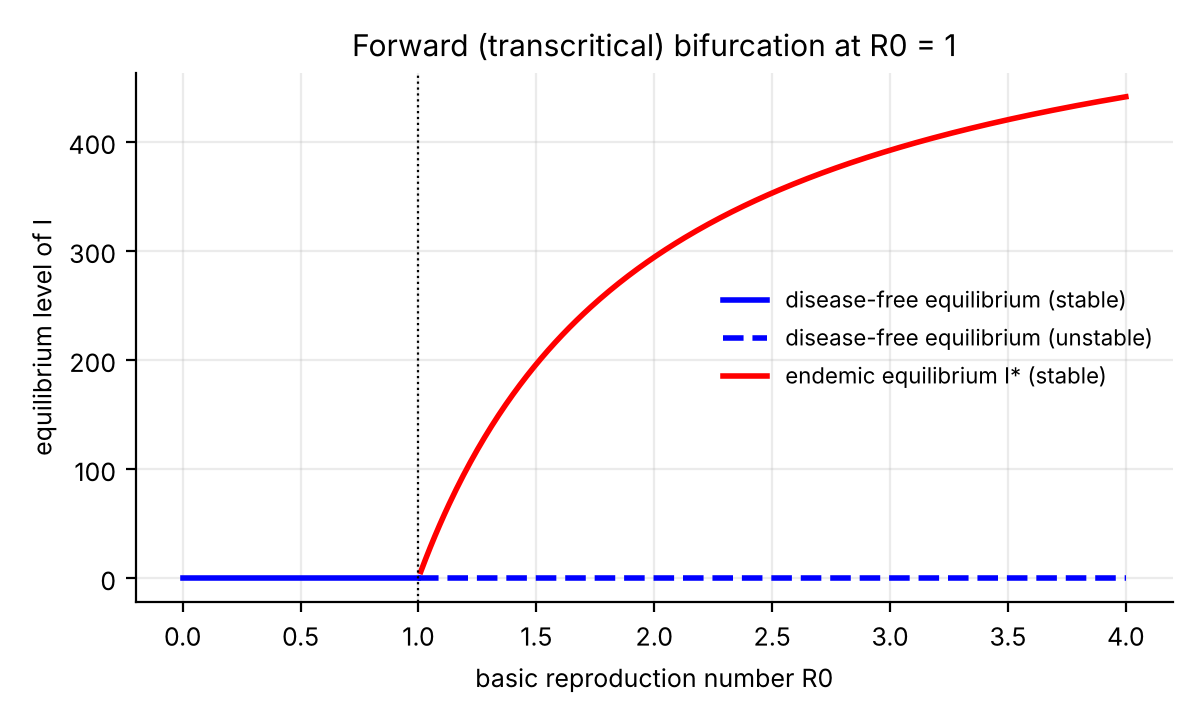
\includegraphics[width=0.9\linewidth]{charts/Fig02_Bifurcation.png}
\caption{Equilibrium level of $I$ against $R_{0}$, computed from the formulas above $(\alpha$, $\gamma$, $\sigma$, $\mu$, A as in Case 1).}
\end{figure}

\section{Numerical Simulation}

The equations were solved numerically for the two cases in Section 6.1 over 365 days (the first 100 days are shown for Case 2, where the infection disappears quickly). A standard ODE solver was used and the results were cross-checked with a spreadsheet implementation of Euler's method with step 0.1 day; the two agree closely (for example the peak of $I$ is 697.9 in the solver and 699.6 in Euler's method). The accompanying Excel workbook, SEIQR\_COVID19\_Simulation.xlsx (Appendix A), reproduces all simulations and lets the reader change the parameters.


Each chart below is shown on its own, followed by an explanation of what it shows and an analysis of why it behaves in this way. The green dashed line marks the equilibrium value and the black dots mark peaks and minima, labelled with their values.


\subsection{Case 1: $R_{0} = 2.35 > 1$}

Parameters: $A = 100$, $\mu = 0.02$, $\beta = 4 \times 10^{-5}$, $\alpha = 0.1$, $\gamma = 0.05$, $\sigma = 0.08$, $\theta = 0.07$, with $S(0) = 4990$, $E(0) = 10$ and $I(0) = Q(0) = R(0) = 0$. Here $R_{0} = 2.353$, so by Theorems 1 and 2 an epidemic occurs and the solution approaches the endemic equilibrium $C^* = (2125.0$, 338.2, 338.2, 488.6, 1710.0).


\subsubsection{Chart 1.1: Susceptible population, $R_{0} = 2.35 > 1$}

\begin{figure}[H]
\centering
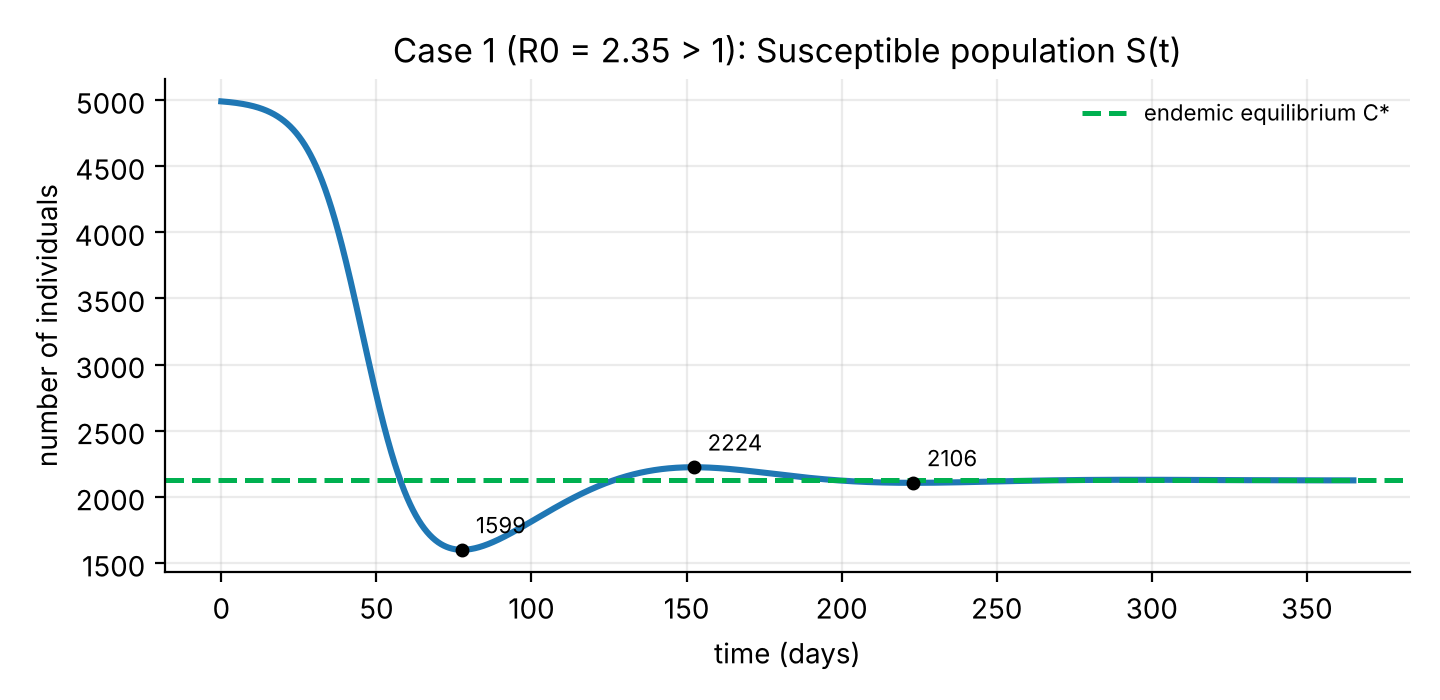
\includegraphics[width=0.9\linewidth]{charts/Fig03_Case1_Susceptible.png}
\caption{Susceptible population $S(t)$ for Case 1 $(R_{0} = 2.35 > 1)$.}
\end{figure}

\textbf{Explanation. }The chart shows how many people remain susceptible over 365 days. $S$ starts at 4990 and hardly changes in the first ten days (4,956 on day 10). It then falls steeply to about 1,989 by day 60 and reaches its minimum of about 1,599 on day 77.6. After that it rises to a small overshoot of about 2,224 near day 152 and oscillates with shrinking swings around the dashed line $S^* =$ 2,125 (2,124.3 on day 365).


\textbf{Analysis. }From $dS/dt = A - \mu S - \beta S(E + I)$, susceptible people are lost through infection at rate $\beta S(E + I)$ and are replaced only by recruitment A. At the start $E + I$ is small, so $S$ barely moves. As exposed and infected people accumulate, the loss term becomes much larger than the inflow and $S$ drops quickly. After the epidemic peak, $E + I$ falls, the loss slows, recruitment pushes $S$ upward and the cycle repeats with smaller swings. This damped oscillation is the effect of the complex eigenvalues \textminus{}0.0229 $\pm$ 0.0441i found in Section 8. In the long run $S^* = N^*/R_{0} =$ 5000/2.353 = 2125, so about 42.5\% of the population stays susceptible.


\subsubsection{Chart 1.2: Exposed population, $R_{0} = 2.35 > 1$}

\begin{figure}[H]
\centering
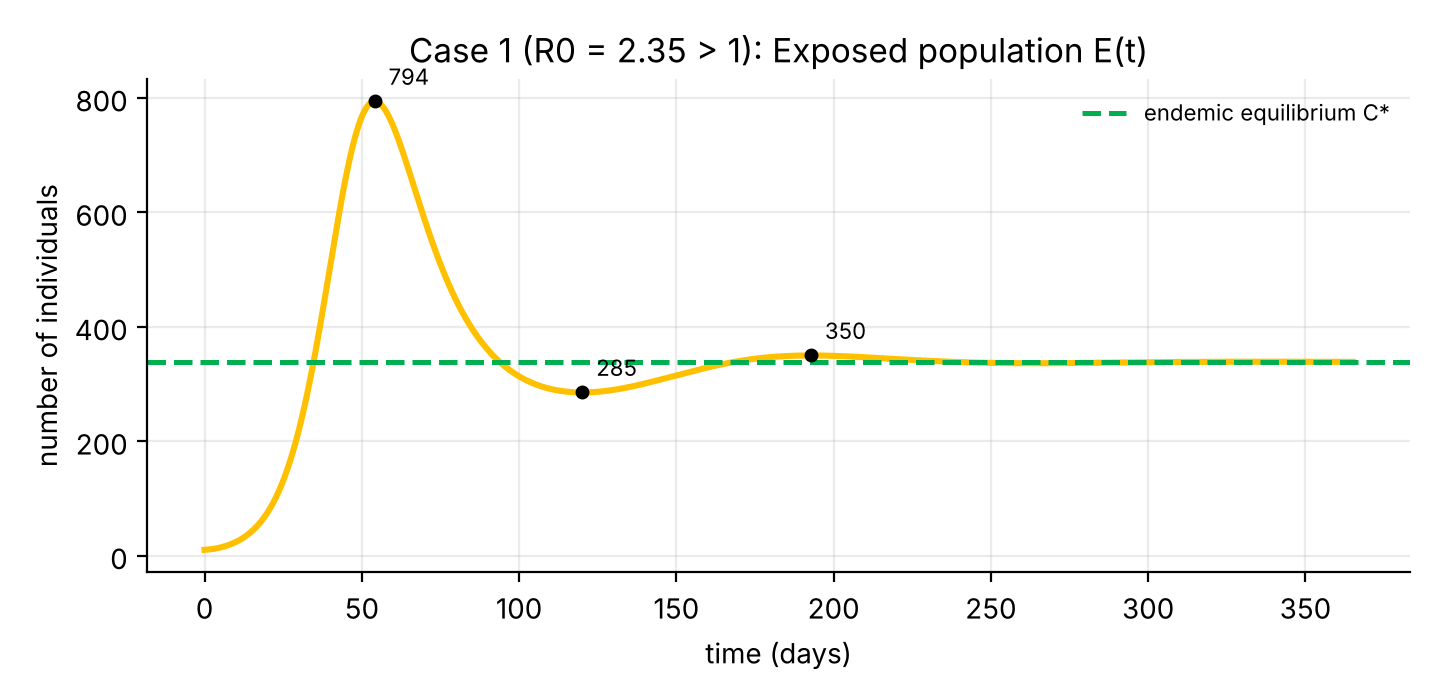
\includegraphics[width=0.9\linewidth]{charts/Fig04_Case1_Exposed.png}
\caption{Exposed population $E(t)$ for Case 1 $(R_{0} = 2.35 > 1)$.}
\end{figure}

\textbf{Explanation. }$E$ starts at 10, grows slowly at first (about 24 on day 10) and then very quickly (220 on day 30, 750 on day 60). It peaks at about 794 on day 54.1, falls to a minimum of about 285 near day 120, rises again to about 350 near day 193 and settles at $E^* = 338$.


\textbf{Analysis. }The equation is $dE/dt = \beta S(E + I) - k_{1}E$. While $S$ is large the gain term exceeds the loss $k_{1}E$, so $E$ grows almost exponentially; this is the behaviour expected when $R_{0} > 1$. The peak occurs when new exposures $\beta S(E + I)$ equal the departures $k_{1}E$, which happens because $S$ has fallen enough (Chart 1.1). After the peak $E$ decreases until $S$ has recovered enough that new exposures again balance departures, giving $E^* = (A/k_{1})(1 - 1/R_{0}) = 338.2$. $E$ peaks about nine days before $I$ (day 54 against day 63.5), because people must be exposed before they can become infected.


\subsubsection{Chart 1.3: Infected population, $R_{0} = 2.35 > 1$}

\begin{figure}[H]
\centering
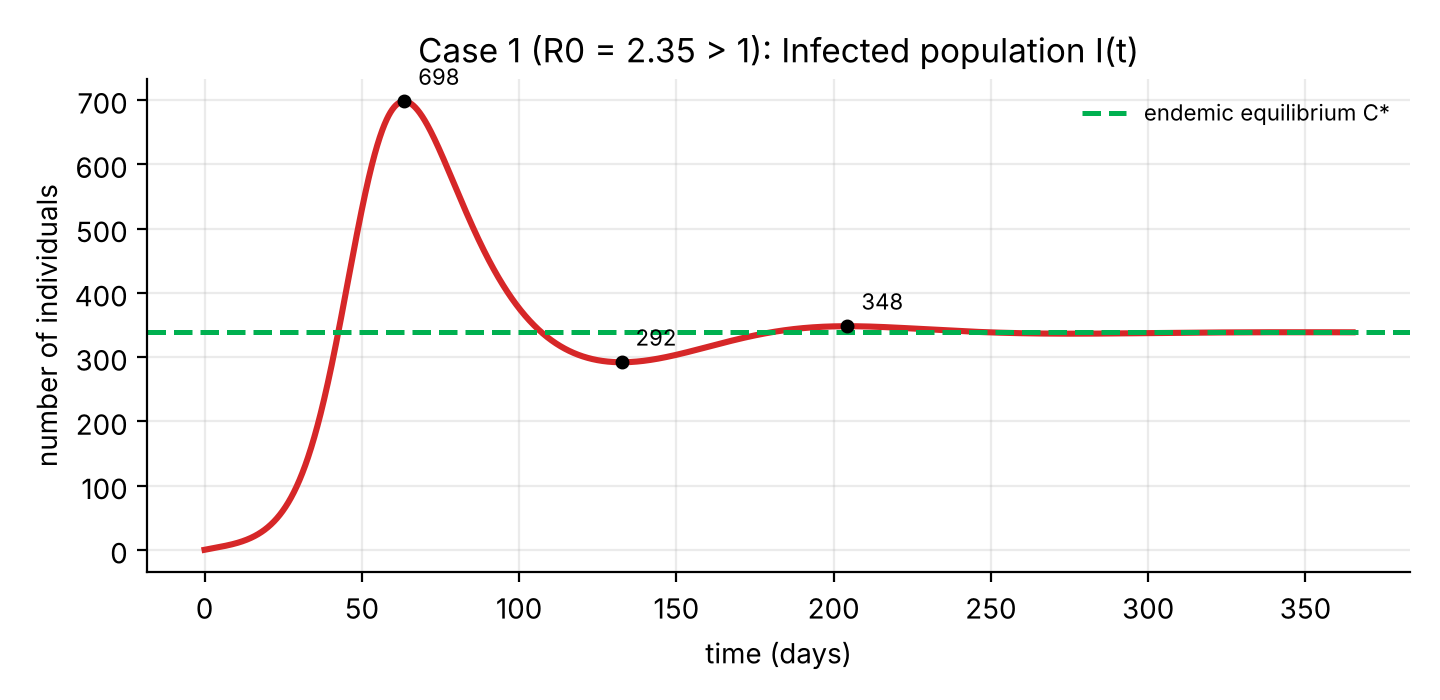
\includegraphics[width=0.9\linewidth]{charts/Fig05_Case1_Infected.png}
\caption{Infected population $I(t)$ for Case 1 $(R_{0} = 2.35 > 1)$.}
\end{figure}

\textbf{Explanation. }$I$ starts at 0 and is still small on day 10 (about 10). It then climbs to about 107 on day 30 and 687 on day 60, and peaks at about 698 on day 63.5. This is the epidemic wave: about 14\% of the population is infected at the same moment. $I$ then falls to about 292 near day 133, rises to about 348 near day 204 and settles at $I^* = 338$.


\textbf{Analysis. }The equation is $dI/dt = \alpha E - k_{2}I$. $I$ grows while exposed people arrive faster than infected people leave (by isolation at rate $\sigma$ or natural death). The peak occurs when $\alpha E = k_{2}I$. Here $\alpha = k_{2} = 0.1$, so the peak is exactly where $E = I$, which is where the two curves cross in Chart 1.6. The later oscillations again come from the complex eigenvalues of Section 8. If only the first 30 days were plotted, $I(t)$ would look like steady growth; the peak and the approach to the endemic level, $I^* = (\alpha /k_{2})E^* = 338$, appear only when the model is run for several months.


\subsubsection{Chart 1.4: Isolated population, $R_{0} = 2.35 > 1$}

\begin{figure}[H]
\centering
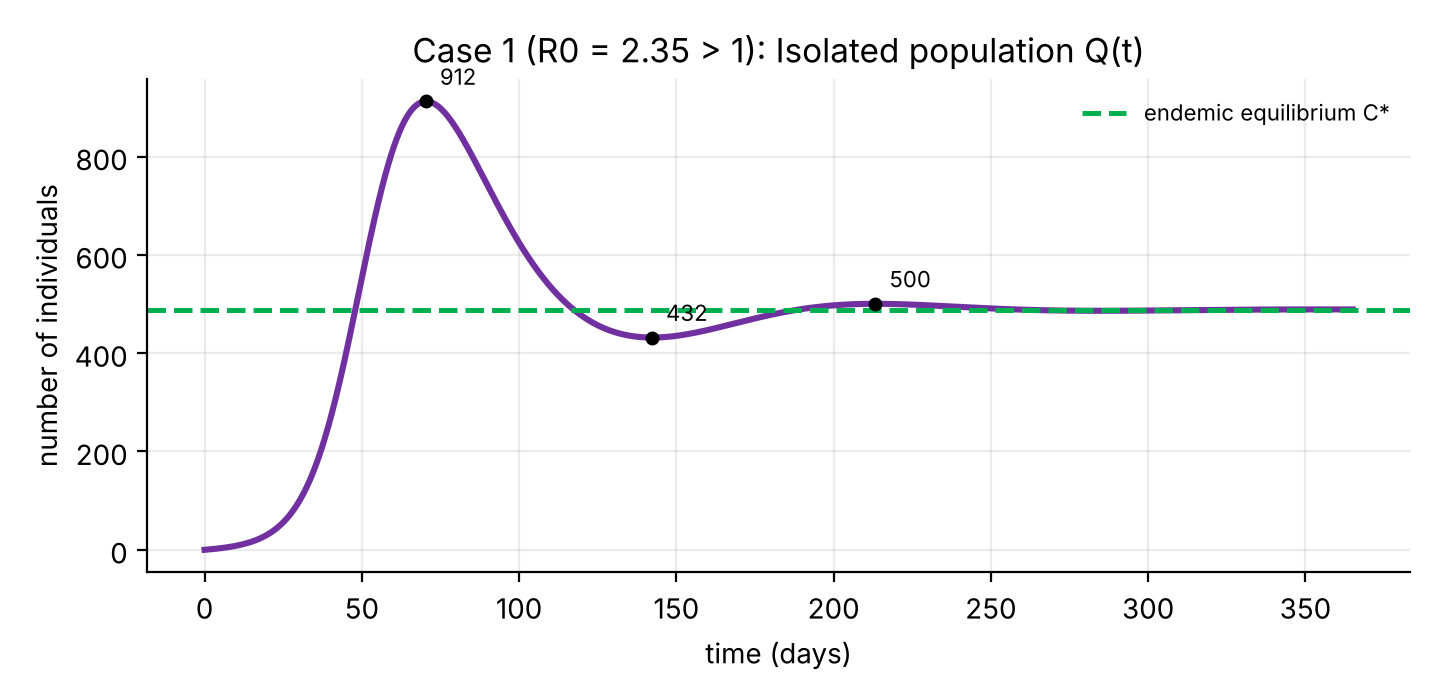
\includegraphics[width=0.9\linewidth]{charts/Fig06_Case1_Isolated.png}
\caption{Isolated population $Q(t)$ for Case 1 $(R_{0} = 2.35 > 1)$.}
\end{figure}

\textbf{Explanation. }$Q$ rises from 0 (about 8 on day 10, 98 on day 30, 817 on day 60) to a peak of about 912 on day 70.4. It falls to about 432 near day 142, rises to about 500 near day 213 and settles at $Q^* = 488.6$.


\textbf{Analysis. }The equation is $dQ/dt = \gamma E + \sigma I - k_{3}Q$. People enter isolation from $E$ (rate $\gamma = 0.05)$ and from $I$ (rate $\sigma = 0.08)$ and leave at rate $k_{3} = \theta + \mu = 0.09$ by recovery or natural death. Because $Q$ is fed by both $E$ and $I$, it peaks after both of them (day 70 against days 54 and 63.5). The peak of 912 is the largest of the three infection classes, so it represents the maximum demand on isolation and care facilities. Isolated people are assumed not to transmit, so every person moved into $Q$ is removed from the chain of transmission.


\subsubsection{Chart 1.5: Recovered population, $R_{0} = 2.35 > 1$}

\begin{figure}[H]
\centering
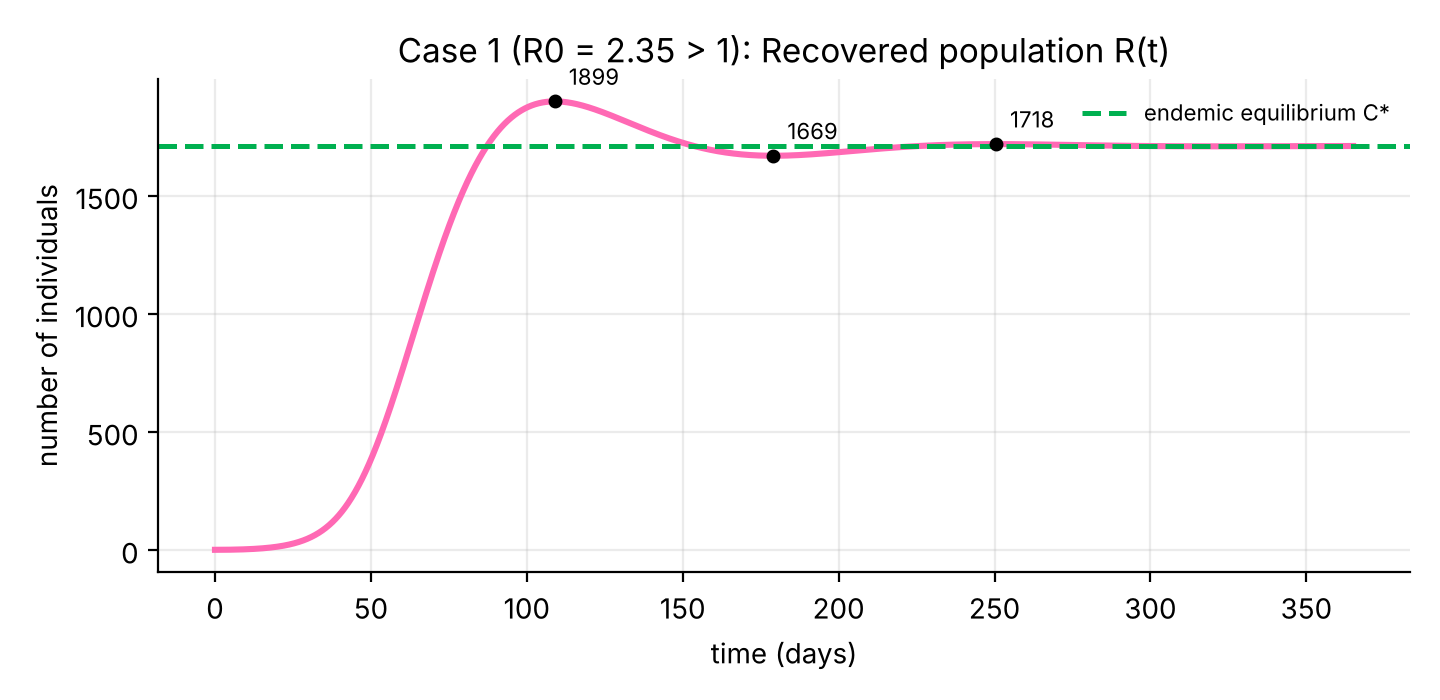
\includegraphics[width=0.9\linewidth]{charts/Fig07_Case1_Recovered.png}
\caption{Recovered population $R(t)$ for Case 1 $(R_{0} = 2.35 > 1)$.}
\end{figure}

\textbf{Explanation. }$R$ grows slowly at first (about 2 on day 10 and 49 on day 30), then quickly (757 on day 60 and 1,873 on day 100). It overshoots to a maximum of about 1,899 on day 109, dips to about 1,669 near day 179 and settles at $R^* =$ 1,710.


\textbf{Analysis. }The equation is $dR/dt = \theta Q - \mu R$. $R$ gains people as isolated individuals recover at rate $\theta = 0.07$ and loses them by natural death at rate $\mu = 0.02$. Because it is fed only by $Q$, $R$ lags behind all other classes. Unlike the classical SIR model, $R$ does not grow for ever: recovered people eventually leave through natural death while newcomers enter $S$, so $R^* = (\theta /\mu )Q^* = 3.5 \times 488.6 = 1710$, which is about 34\% of the population. In the long run the population is divided as $S$ 42.5\%, $E$ 6.8\%, $I$ 6.8\%, $Q$ 9.8\% and $R$ 34.2\%.


\subsubsection{Chart 1.6: Exposed, infected and isolated together, $R_{0} = 2.35 > 1$}

\begin{figure}[H]
\centering
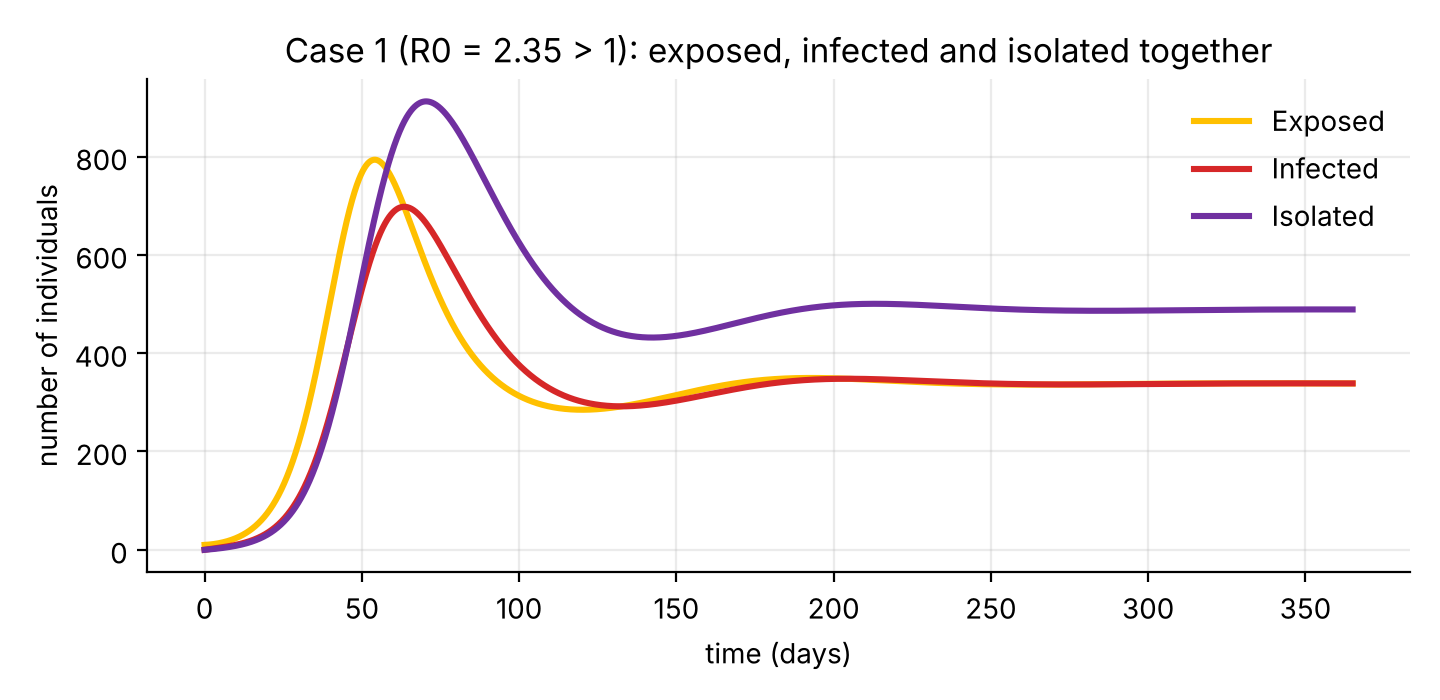
\includegraphics[width=0.9\linewidth]{charts/Fig08_Case1_E_I_Q_together.png}
\caption{Exposed, infected and isolated populations together for Case 1.}
\end{figure}

\textbf{Explanation. }The three infection classes are drawn on the same axes. They form one wave that passes through the stages in order: $E$ peaks first (day 54, about 794), then $I$ (day 63.5, about 698) and then $Q$ (day 70, about 912). After the wave all three oscillate and settle at $E^* = I^* = 338$ and $Q^* = 489$.


\textbf{Analysis. }The delay between the peaks reflects the flow $E \to I \to Q$ in Figure 1: each class is fed by the one before it. $E^*$ and $I^*$ are equal because $\alpha = k_{2}$, so $I^* = (\alpha /k_{2})E^* = E^*$. $Q^*$ is larger than both because isolated people stay in the class for $1/k_{3} \approx 11$ days and are fed from both $E$ and $I$. The chart also shows that the disease does not disappear but remains at a steady level; this is the endemic state predicted for $R_{0} > 1$.


The key numbers for Case 1 are collected in the table below.


\begin{longtable}{>{\raggedright\arraybackslash}p{\dimexpr(\linewidth-4\tabcolsep)*4200/9026\relax}>{\raggedright\arraybackslash}p{\dimexpr(\linewidth-4\tabcolsep)*4826/9026\relax}}
\hline
\rowcolor[HTML]{D9E2F3}\textbf{Quantity (Case 1)} & \textbf{Value} \\ \hline
\endhead
Peak of $E$ & 793.6 on day 54.1 \\ \hline
Peak of $I$ & 697.9 on day 63.5 \\ \hline
Peak of $Q$ & 912.3 on day 70.4 \\ \hline
Minimum of $S$ & 1599 on day 77.6 \\ \hline
Maximum of $R$ & 1899 on day 109 \\ \hline
Endemic equilibrium $C^* (S$, $E$, $I$, $Q$, $R)$ & 2125.0, 338.2, 338.2, 488.6, 1710.0 \\ \hline
State on day 365 $(S$, $E$, $I$, $Q$, $R)$ & 2124.3, 338.4, 338.5, 489.0, 1709.9 \\ \hline
\end{longtable}

\subsection{Case 2: $R_{0} = 0.59 < 1$}

Parameters: the same as Case 1 except $\beta = 1 \times 10^{-5}$, so $R_{0} = 0.588$. By Theorem 1 the disease-free equilibrium $C_{0} = (5000$, 0, 0, 0, 0) is stable and the infection should die out. The charts show the first 100 days.


\subsubsection{Chart 2.1: Susceptible population, $R_{0} = 0.59 < 1$}

\begin{figure}[H]
\centering
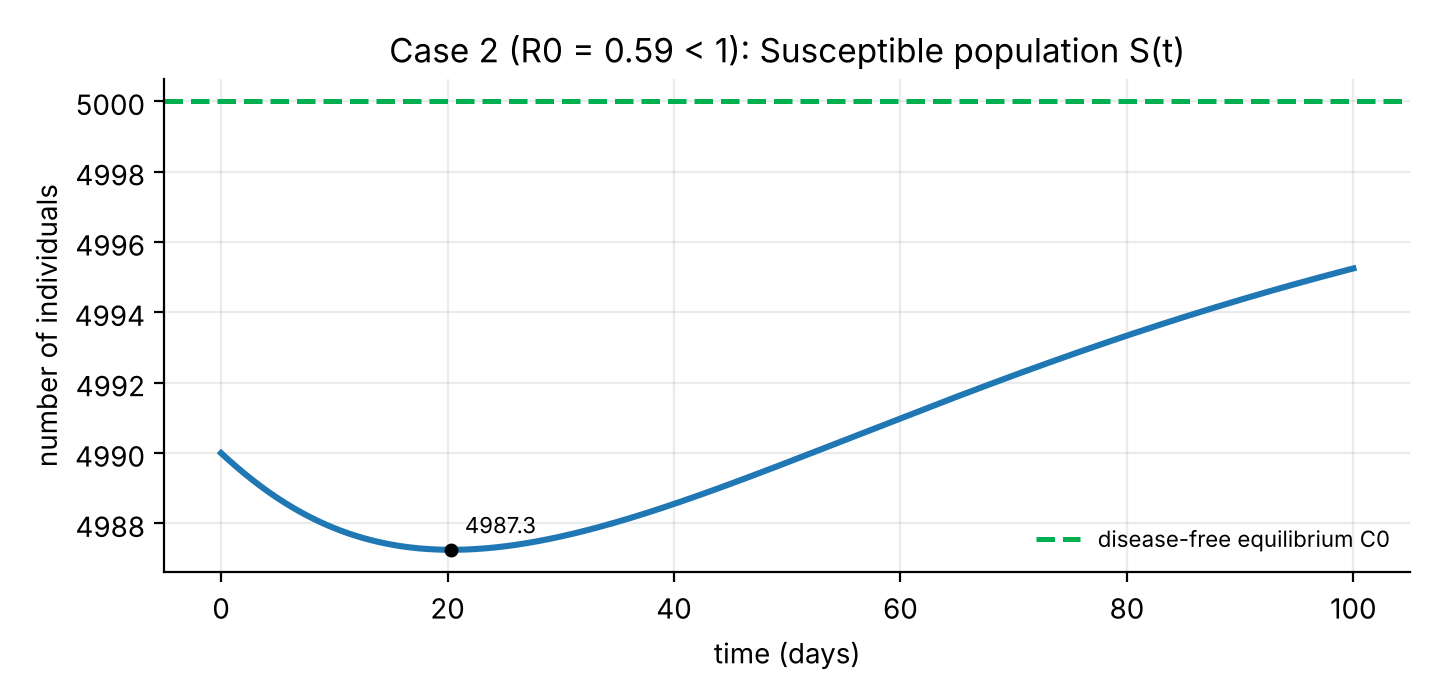
\includegraphics[width=0.9\linewidth]{charts/Fig09_Case2_Susceptible.png}
\caption{Susceptible population $S(t)$ for Case 2 $(R_{0} = 0.59 < 1)$.}
\end{figure}

\textbf{Explanation. }$S$ starts at 4990 and dips only slightly, to about 4,987 near day 20. It then rises steadily back towards the dashed line $N^* = 5000$ (4,995 on day 100).


\textbf{Analysis. }With a small transmission rate the infection term $\beta S(E + I)$ removes only a handful of people from $S$. At the same time the people who were initially exposed, infected or recovered gradually leave the population by natural death and are replaced by new susceptible recruits (rate A). Therefore $S$ returns to $A/\mu = 5000$, which is the susceptible level of the disease-free equilibrium $C_{0}$. The very small dip of about 3 people shows that almost nobody is infected, in contrast with Chart 1.1.


\subsubsection{Chart 2.2: Exposed population, $R_{0} = 0.59 < 1$}

\begin{figure}[H]
\centering
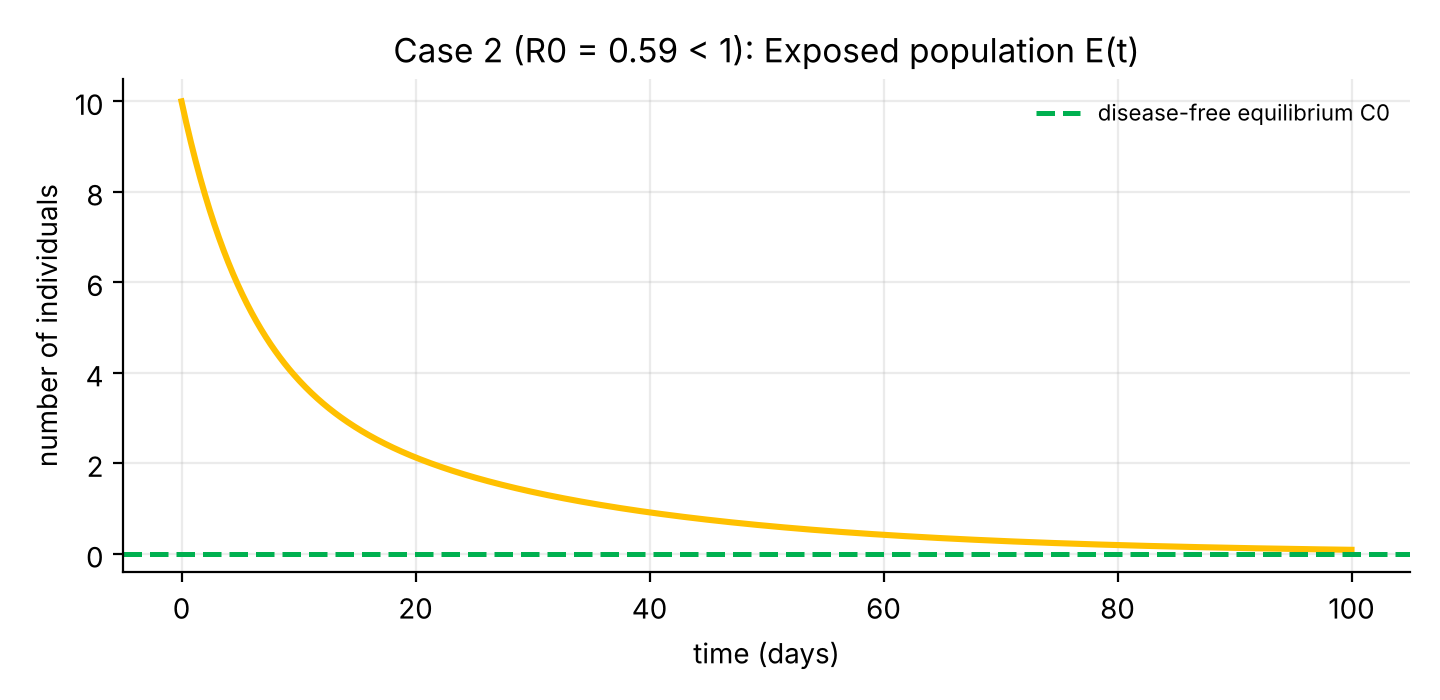
\includegraphics[width=0.9\linewidth]{charts/Fig10_Case2_Exposed.png}
\caption{Exposed population $E(t)$ for Case 2 $(R_{0} = 0.59 < 1)$.}
\end{figure}

\textbf{Explanation. }$E$ decreases from its initial value of 10 and never rises: it is about 5.8 on day 5, 2.1 on day 20, 0.6 on day 50 and 0.09 on day 100.


\textbf{Analysis. }In $dE/dt = \beta S(E + I) - k_{1}E$ the new exposures are always smaller than the departures $k_{1}E$, because $R_{0} < 1$: one case produces less than one new case. $E$ therefore decays, quickly at first and then more slowly. In the later part the decay follows the dominant eigenvalue \textminus{}0.0386 found in Section 7: from day 50 to day 100 the value drops by the factor $e^{-0.0386 \times 50} \approx 0.145$, which agrees with 0.09/0.62. The corresponding half-life is about 18 days.


\subsubsection{Chart 2.3: Infected population, $R_{0} = 0.59 < 1$}

\begin{figure}[H]
\centering
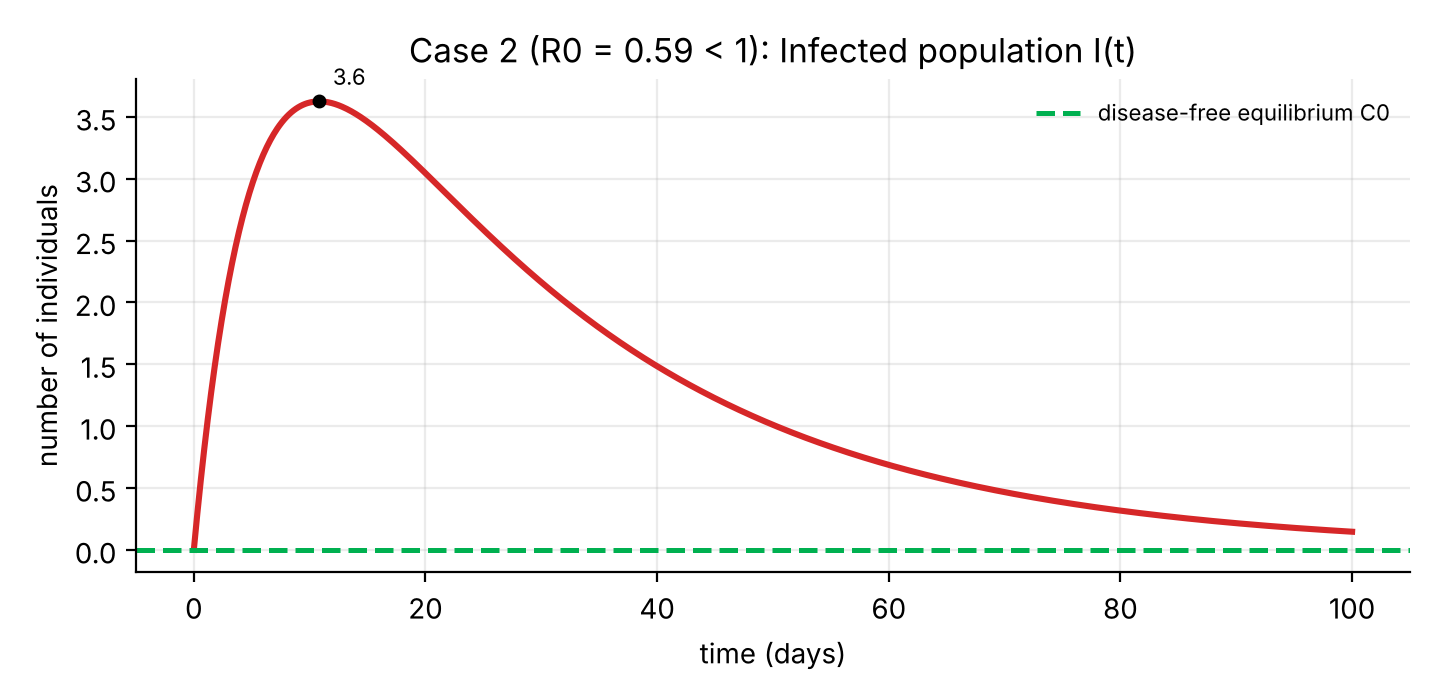
\includegraphics[width=0.9\linewidth]{charts/Fig11_Case2_Infected.png}
\caption{Infected population $I(t)$ for Case 2 $(R_{0} = 0.59 < 1)$.}
\end{figure}

\textbf{Explanation. }$I$ rises from 0 to a small maximum of about 3.6 on day 10.8 and then decays: about 1.0 on day 50 and 0.15 on day 100.


\textbf{Analysis. }In $dI/dt = \alpha E - k_{2}I$ the first term is positive at the start because 10 people are exposed and move into $I$ at rate $\alpha = 0.1$, so $I$ rises briefly. As $E$ shrinks the inflow falls, and $I$ peaks when $\alpha E = k_{2}I$, that is when $E = I$ (the curves cross near day 11 in Chart 2.6). This small bump is only the initial transient caused by the 10 starting exposed individuals. There is no epidemic wave: the maximum is 3.6 infected people, compared with 698 in Case 1.


\subsubsection{Chart 2.4: Isolated population, $R_{0} = 0.59 < 1$}

\begin{figure}[H]
\centering
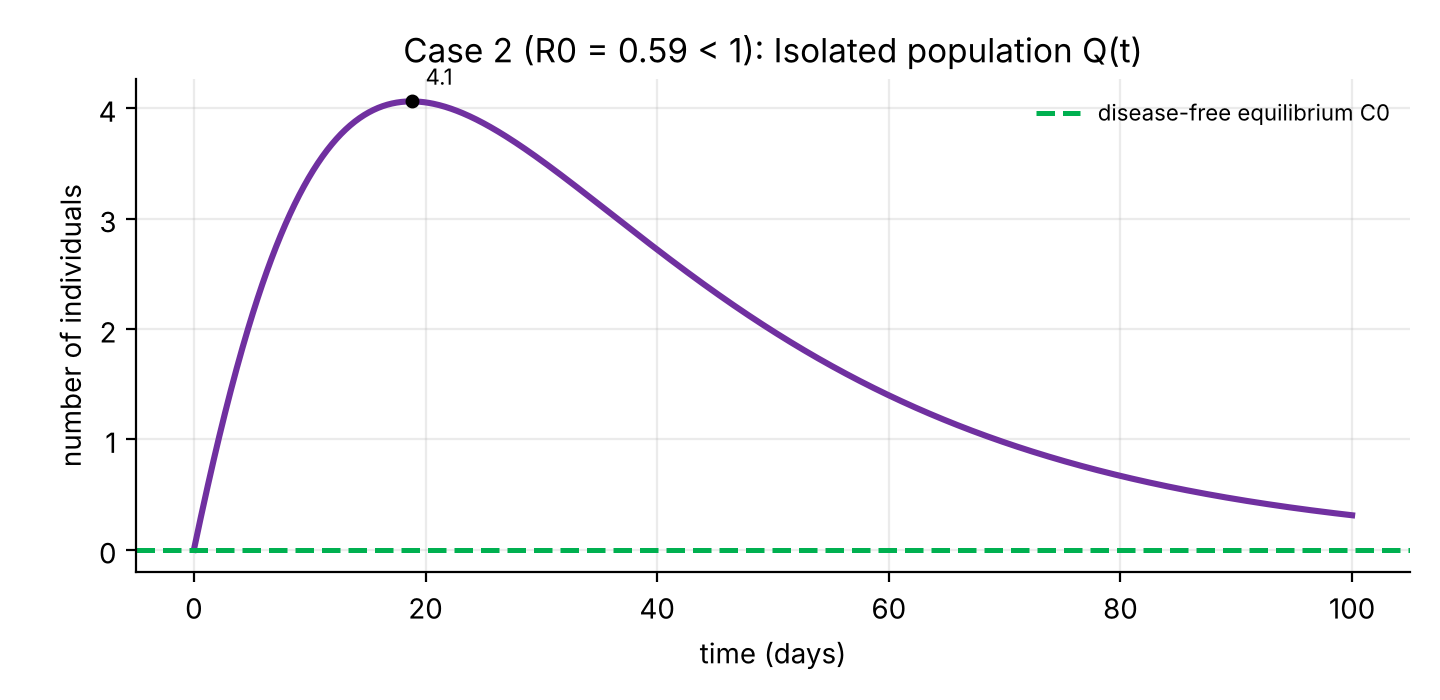
\includegraphics[width=0.9\linewidth]{charts/Fig12_Case2_Isolated.png}
\caption{Isolated population $Q(t)$ for Case 2 $(R_{0} = 0.59 < 1)$.}
\end{figure}

\textbf{Explanation. }$Q$ increases to a small maximum of about 4.1 on day 18.8 and then falls: about 2.0 on day 50 and 0.3 on day 100.


\textbf{Analysis. }$Q$ is fed by $\gamma E + \sigma I$ and drained at rate $k_{3} = 0.09$. Since $E$ and $I$ are both small and decreasing, the inflow soon drops below the outflow and $Q$ decays. Its peak comes after the peak of $I$, as the flow $E \to I \to Q$ suggests. The largest number of isolated people is about 4, more than 200 times smaller than the peak of 912 in Case 1, so with $R_{0} < 1$ the demand on isolation facilities is negligible.


\subsubsection{Chart 2.5: Recovered population, $R_{0} = 0.59 < 1$}

\begin{figure}[H]
\centering
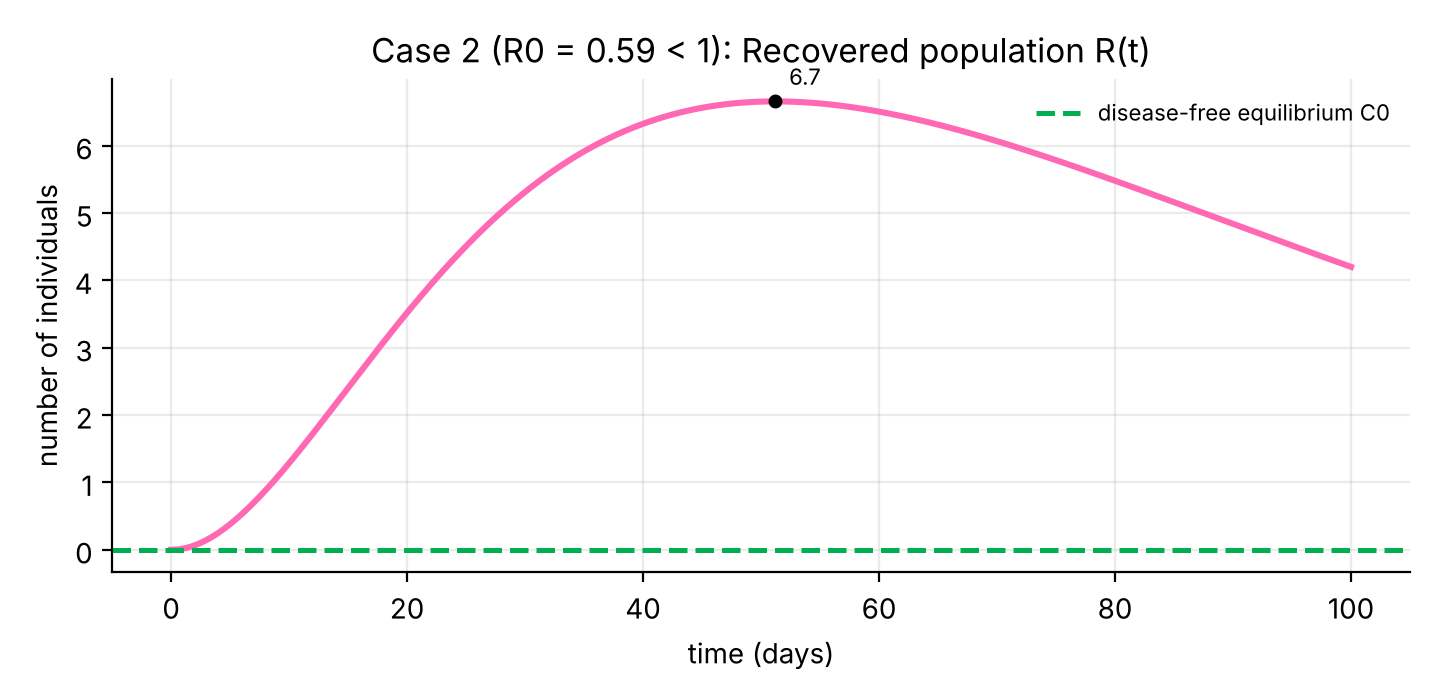
\includegraphics[width=0.9\linewidth]{charts/Fig13_Case2_Recovered.png}
\caption{Recovered population $R(t)$ for Case 2 $(R_{0} = 0.59 < 1)$.}
\end{figure}

\textbf{Explanation. }$R$ grows slowly to a maximum of about 6.7 near day 51 (1.3 on day 10, 5.3 on day 30) and then declines (4.2 on day 100) towards zero.


\textbf{Analysis. }In $dR/dt = \theta Q - \mu R$, recovered people are added only while $Q$ is non-zero and they leave by natural death at rate $\mu = 0.02$. When $Q$ has become very small the loss term dominates and $R$ decays. At the disease-free equilibrium $R = 0$, because there are no infections and the small number of people who recovered have been replaced by newcomers. This differs from Case 1, where $R$ settles at a large positive value (1710).


\subsubsection{Chart 2.6: Exposed, infected and isolated together, $R_{0} = 0.59 < 1$}

\begin{figure}[H]
\centering
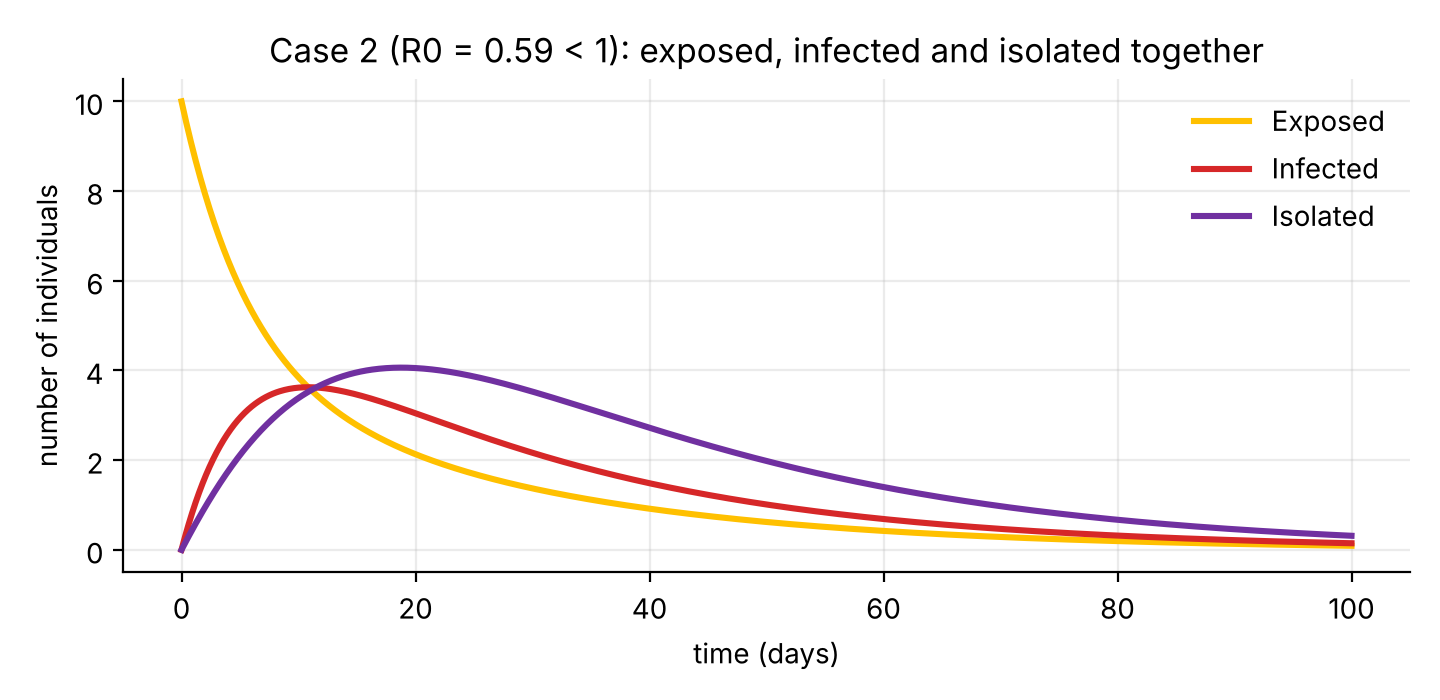
\includegraphics[width=0.9\linewidth]{charts/Fig14_Case2_E_I_Q_together.png}
\caption{Exposed, infected and isolated populations together for Case 2.}
\end{figure}

\textbf{Explanation. }All three classes end at zero. $E$ decreases from the start, $I$ peaks at about 3.6 on day 10.8 and $Q$ at about 4.1 on day 18.8, and all three fall below one person within about 70 days. By day 365 all are zero to numerical accuracy.


\textbf{Analysis. }This chart summarises the meaning of $R_{0} < 1$. The infection passes through the same stages as in Case 1 but each class is smaller than the one before it in time and nothing sustains the chain. All classes decay at the rate set by the eigenvalues \textminus{}0.0386 and \textminus{}0.1814 of the infection block, so the disease disappears without any outbreak. Compare Chart 1.6, where the three classes rise to hundreds and then persist.


\subsection{Phase plane}

A phase-plane chart plots two variables against each other (here $S$ against $I)$ instead of plotting each against time. Each curve is one solution; the black dot is its starting point. Five different initial states are shown in each chart.


\subsubsection{Chart 3.1: S–I phase plane, $R_{0} = 2.35 > 1$}

\begin{figure}[H]
\centering
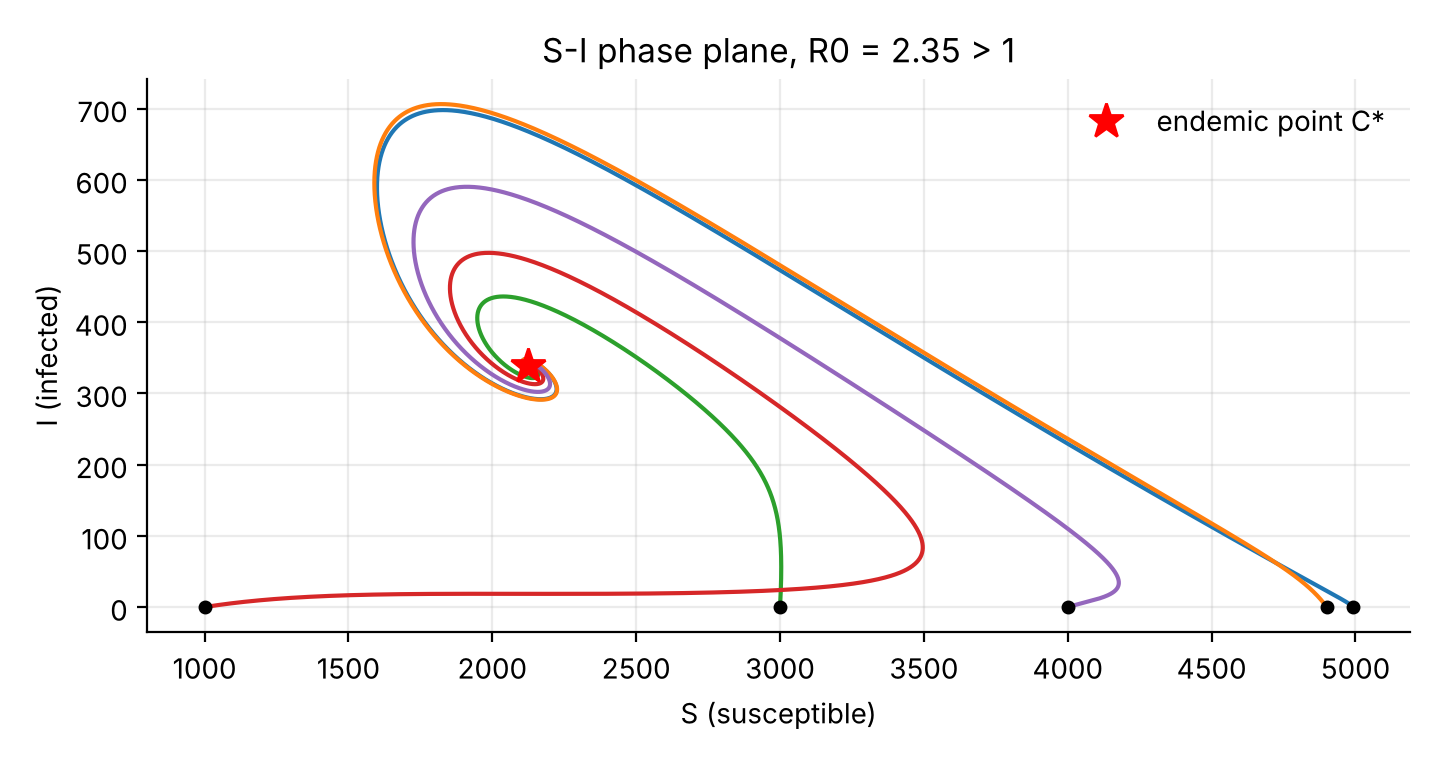
\includegraphics[width=0.9\linewidth]{charts/Fig15_PhasePlane_Case1.png}
\caption{S–I phase plane for Case 1 $(R_{0} = 2.35 > 1)$.}
\end{figure}

\textbf{Explanation. }Every curve leaves its starting point, moves to the left $(S$ falls) while $I$ rises, reaches a maximum of $I$ and then curls around and winds inward to the red star, the endemic point $C^* \approx (2125$, 338).


\textbf{Analysis. }The curves do not go back to the disease-free point $(S = 5000$, $I = 0)$. This confirms Theorem 1: for $R_{0} > 1$ the disease-free equilibrium is unstable, so trajectories starting near it move away. The inward spiralling around $C^*$ confirms Theorem 2: $C^*$ is stable, and the spiral shape comes from its complex eigenvalues. Different starting states lead to the same endemic point, so the long-run behaviour does not depend on the initial numbers.


\subsubsection{Chart 3.2: S–I phase plane, $R_{0} = 0.59 < 1$}

\begin{figure}[H]
\centering
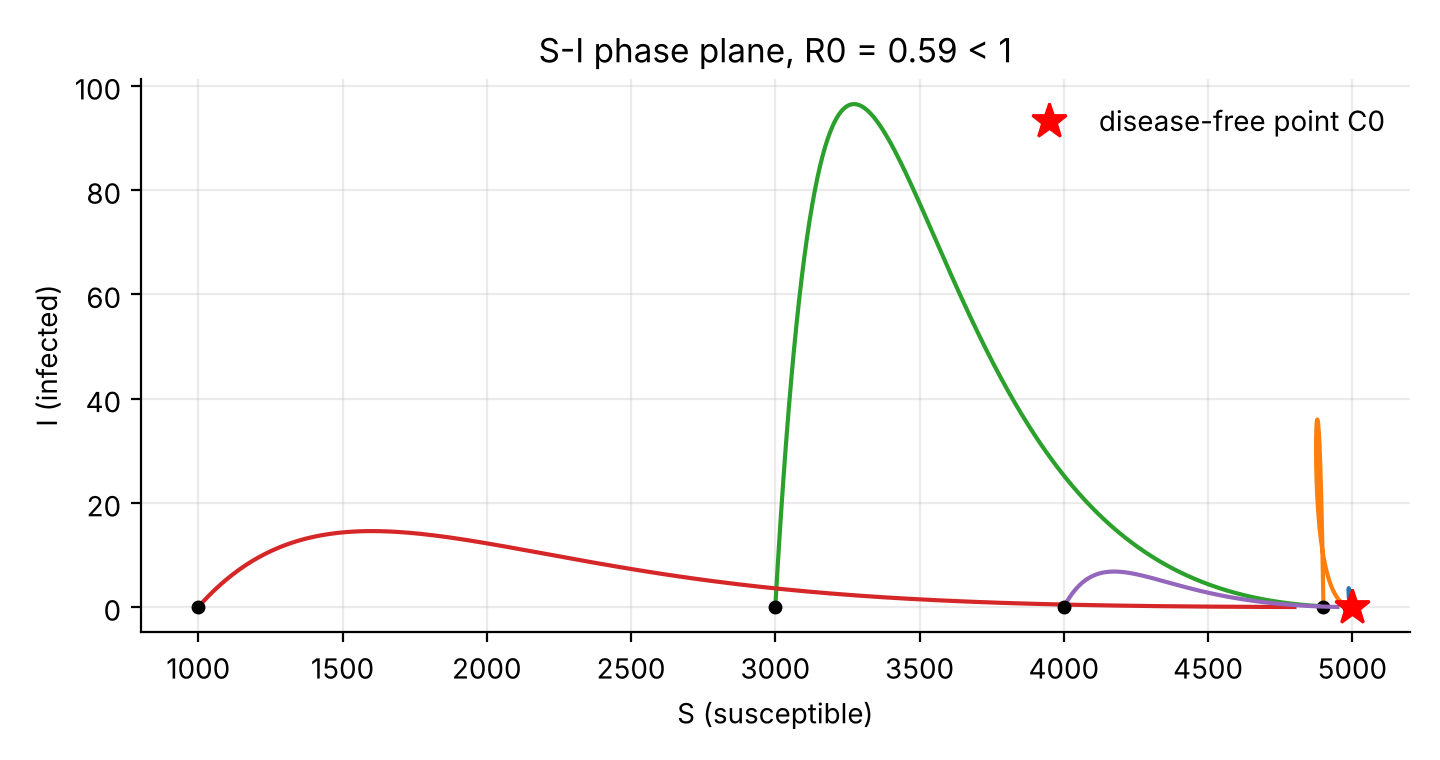
\includegraphics[width=0.9\linewidth]{charts/Fig16_PhasePlane_Case2.png}
\caption{S–I phase plane for Case 2 $(R_{0} = 0.59 < 1)$.}
\end{figure}

\textbf{Explanation. }All five curves end at the red star, the disease-free point $(S = 5000$, $I = 0)$. Curves that start with many exposed people (for example $E(0) = 300)$ first show a short rise in $I$, which then collapses back to zero.


\textbf{Analysis. }This agrees with Theorem 1 for $R_{0} < 1$: the disease-free equilibrium attracts the solutions. The temporary rise in $I$ for large starting $E$ is a transient, since 300 initially exposed people have to pass through $I$ before they are removed. Because each infected person produces fewer than one new case, the rise cannot be sustained.


\section{Effect of Isolation on $R_{0}$ and on the Outbreak}

Since $\gamma$ appears only in $k_{1}$ and $\sigma$ only in $k_{2}$, differentiating $R_{0}$ gives


\begin{equation}
\frac{\partial R_0}{\partial\gamma} = -\frac{\beta N^*(k_2+\alpha)}{k_1^2k_2} < 0,\qquad \frac{\partial R_0}{\partial\sigma} = -\frac{\beta N^*\alpha}{k_1k_2^2} < 0
\end{equation}

so faster isolation always lowers $R_{0}$. Table 1 shows $R_{0}$ for several values of $\gamma$ and $\sigma$ with $\beta = 4 \times 10^{-5}$; shaded cells have $R_{0} < 1$.


\begin{longtable}{>{\raggedright\arraybackslash}p{\dimexpr(\linewidth-14\tabcolsep)*1226/9026\relax}>{\centering\arraybackslash}p{\dimexpr(\linewidth-14\tabcolsep)*1300/9026\relax}>{\centering\arraybackslash}p{\dimexpr(\linewidth-14\tabcolsep)*1300/9026\relax}>{\centering\arraybackslash}p{\dimexpr(\linewidth-14\tabcolsep)*1300/9026\relax}>{\centering\arraybackslash}p{\dimexpr(\linewidth-14\tabcolsep)*1300/9026\relax}>{\centering\arraybackslash}p{\dimexpr(\linewidth-14\tabcolsep)*1300/9026\relax}>{\centering\arraybackslash}p{\dimexpr(\linewidth-14\tabcolsep)*1300/9026\relax}}
\hline
\rowcolor[HTML]{D9E2F3}\textbf{$\gamma \setminus \sigma$} & \textbf{0.00} & \textbf{0.08} & \textbf{0.20} & \textbf{0.40} & \textbf{0.60} & \textbf{1.00} \\ \hline
\endhead
0.00 & \cellcolor[HTML]{FCE4D6}10.00 & \cellcolor[HTML]{FCE4D6}3.33 & \cellcolor[HTML]{FCE4D6}2.42 & \cellcolor[HTML]{FCE4D6}2.06 & \cellcolor[HTML]{FCE4D6}1.94 & \cellcolor[HTML]{FCE4D6}1.83 \\ \hline
0.05 & \cellcolor[HTML]{FCE4D6}7.06 & \cellcolor[HTML]{FCE4D6}2.35 & \cellcolor[HTML]{FCE4D6}1.71 & \cellcolor[HTML]{FCE4D6}1.46 & \cellcolor[HTML]{FCE4D6}1.37 & \cellcolor[HTML]{FCE4D6}1.29 \\ \hline
0.10 & \cellcolor[HTML]{FCE4D6}5.45 & \cellcolor[HTML]{FCE4D6}1.82 & \cellcolor[HTML]{FCE4D6}1.32 & \cellcolor[HTML]{FCE4D6}1.13 & \cellcolor[HTML]{FCE4D6}1.06 & \cellcolor[HTML]{C6EFCE}0.998 \\ \hline
0.20 & \cellcolor[HTML]{FCE4D6}3.75 & \cellcolor[HTML]{FCE4D6}1.25 & \cellcolor[HTML]{C6EFCE}0.91 & \cellcolor[HTML]{C6EFCE}0.77 & \cellcolor[HTML]{C6EFCE}0.73 & \cellcolor[HTML]{C6EFCE}0.69 \\ \hline
0.30 & \cellcolor[HTML]{FCE4D6}2.86 & \cellcolor[HTML]{C6EFCE}0.95 & \cellcolor[HTML]{C6EFCE}0.69 & \cellcolor[HTML]{C6EFCE}0.59 & \cellcolor[HTML]{C6EFCE}0.55 & \cellcolor[HTML]{C6EFCE}0.52 \\ \hline
0.50 & \cellcolor[HTML]{FCE4D6}1.94 & \cellcolor[HTML]{C6EFCE}0.65 & \cellcolor[HTML]{C6EFCE}0.47 & \cellcolor[HTML]{C6EFCE}0.40 & \cellcolor[HTML]{C6EFCE}0.37 & \cellcolor[HTML]{C6EFCE}0.35 \\ \hline
\end{longtable}

\begin{center}\small\textbf{Table 1:} $R_{0}$ as a function of the isolation rates $\gamma$ and $\sigma (\beta = 4 \times 10^{-5}$, $\alpha = 0.1$, $\mu = 0.02$, $A = 100)$.\end{center}

Two conclusions follow. First, with $\sigma = 0.08$ the isolation rate of exposed people must reach $\gamma = 0.28$ for $R_{0} = 1$. Second, as $\sigma \to \infty$ we have $R_{0} \to \beta N^*/k_{1}$, so if $\gamma \le \beta N^* - \alpha - \mu$ (here 0.08) no isolation of infected people alone can bring $R_{0}$ below 1. This happens because exposed people also transmit; identifying and isolating exposed people (testing and contact tracing) is essential.


\begin{figure}[H]
\centering
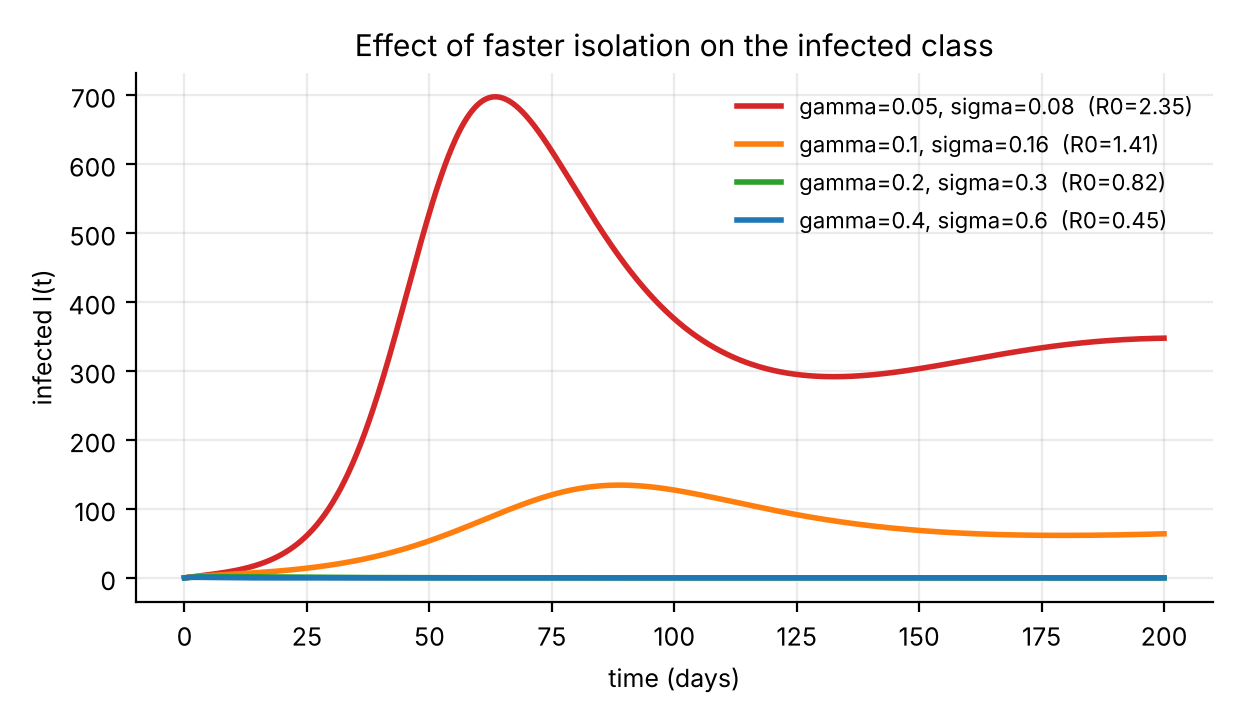
\includegraphics[width=0.9\linewidth]{charts/Fig17_Isolation_Effect.png}
\caption{Infected class for four levels of isolation $(\beta = 4 \times 10^{-5})$.}
\end{figure}

\begin{longtable}{>{\raggedright\arraybackslash}p{\dimexpr(\linewidth-8\tabcolsep)*2300/9026\relax}>{\centering\arraybackslash}p{\dimexpr(\linewidth-8\tabcolsep)*1400/9026\relax}>{\raggedright\arraybackslash}p{\dimexpr(\linewidth-8\tabcolsep)*3326/9026\relax}>{\centering\arraybackslash}p{\dimexpr(\linewidth-8\tabcolsep)*2000/9026\relax}}
\hline
\rowcolor[HTML]{D9E2F3}\textbf{Isolation rates $(\gamma$, $\sigma )$} & \textbf{$R_{0}$} & \textbf{Peak of $I$} & \textbf{Day of peak} \\ \hline
\endhead
0.05, 0.08 (baseline) & 2.35 & 697.9 & 63.5 \\ \hline
0.10, 0.16 & 1.41 & 134.6 & 88.9 \\ \hline
0.20, 0.30 & 0.82 & no epidemic (max 1.9, initial transient) & – \\ \hline
0.40, 0.60 & 0.45 & no epidemic (max 0.8, initial transient) & – \\ \hline
\end{longtable}

Doubling the isolation rates cuts the epidemic peak from about 698 to about 135 and delays it by about 25 days; when $R_{0}$ falls below 1 there is no epidemic wave at all.


\section{Sensitivity Analysis of $R_{0}$}

$R_{0}$ depends on seven parameters. To find which ones matter most we use the normalised forward sensitivity index \cite{r14},


\begin{equation}
\Upsilon_p = \frac{\partial R_0}{\partial p}\cdot\frac{p}{R_0}
\end{equation}

A value $\Upsilon _{p} =$ +0.4 means that a 1\% increase in $p$ raises $R_{0}$ by about 0.4\%; a negative value means that $R_{0}$ falls. Taking logarithms of $R_{0} = (\beta A/\mu )(k_{2} + \alpha )/(k_{1}k_{2})$,


\begin{equation*}
\ln R_0 = \ln\beta+\ln A-\ln\mu+\ln(\sigma+\mu+\alpha)-\ln(\alpha+\mu+\gamma)-\ln(\sigma+\mu)
\end{equation*}

and differentiating with respect to each parameter gives


\begin{equation}
\Upsilon_\beta = \Upsilon_A = 1,\qquad \Upsilon_\theta = 0
\end{equation}

\begin{equation}
\Upsilon_\gamma = -\frac{\gamma}{k_1},\qquad \Upsilon_\sigma = \sigma\left[\frac{1}{k_2+\alpha}-\frac{1}{k_2}\right]
\end{equation}

\begin{equation}
\Upsilon_\alpha = \alpha\left[\frac{1}{k_2+\alpha}-\frac{1}{k_1}\right],\qquad \Upsilon_\mu = -1+\frac{\mu}{k_2+\alpha}-\frac{\mu}{k_1}-\frac{\mu}{k_2}
\end{equation}

These formulas were also checked numerically by changing each parameter by $\pm$0.1\%. For Case 1 $(R_{0} = 2.353)$ the indices are:


\begin{longtable}{>{\raggedright\arraybackslash}p{\dimexpr(\linewidth-6\tabcolsep)*2000/9026\relax}>{\centering\arraybackslash}p{\dimexpr(\linewidth-6\tabcolsep)*1800/9026\relax}>{\raggedright\arraybackslash}p{\dimexpr(\linewidth-6\tabcolsep)*5226/9026\relax}}
\hline
\rowcolor[HTML]{D9E2F3}\textbf{Parameter} & \textbf{Index $\Upsilon$} & \textbf{Meaning} \\ \hline
\endhead
$\beta$ & +1.000 & $R_{0}$ is proportional to the transmission rate. \\ \hline
A & +1.000 & $R_{0}$ is proportional to the recruitment rate (through $N^* = A/\mu )$. \\ \hline
$\mu$ & \textminus{}1.218 & A larger death rate reduces $N^*$ and shortens every stage. \\ \hline
$\sigma$ & \textminus{}0.400 & Faster isolation of infected people lowers $R_{0}$. \\ \hline
$\gamma$ & \textminus{}0.294 & Faster isolation of exposed people lowers $R_{0}$. \\ \hline
$\alpha$ & \textminus{}0.088 & Faster progression $E \to I$ lowers $R_{0}$ slightly. \\ \hline
$\theta$ & 0.000 & $R_{0}$ does not depend on the recovery rate. \\ \hline
\end{longtable}

\subsubsection{Chart 4.1: Sensitivity indices of $R_{0}$}

\begin{figure}[H]
\centering
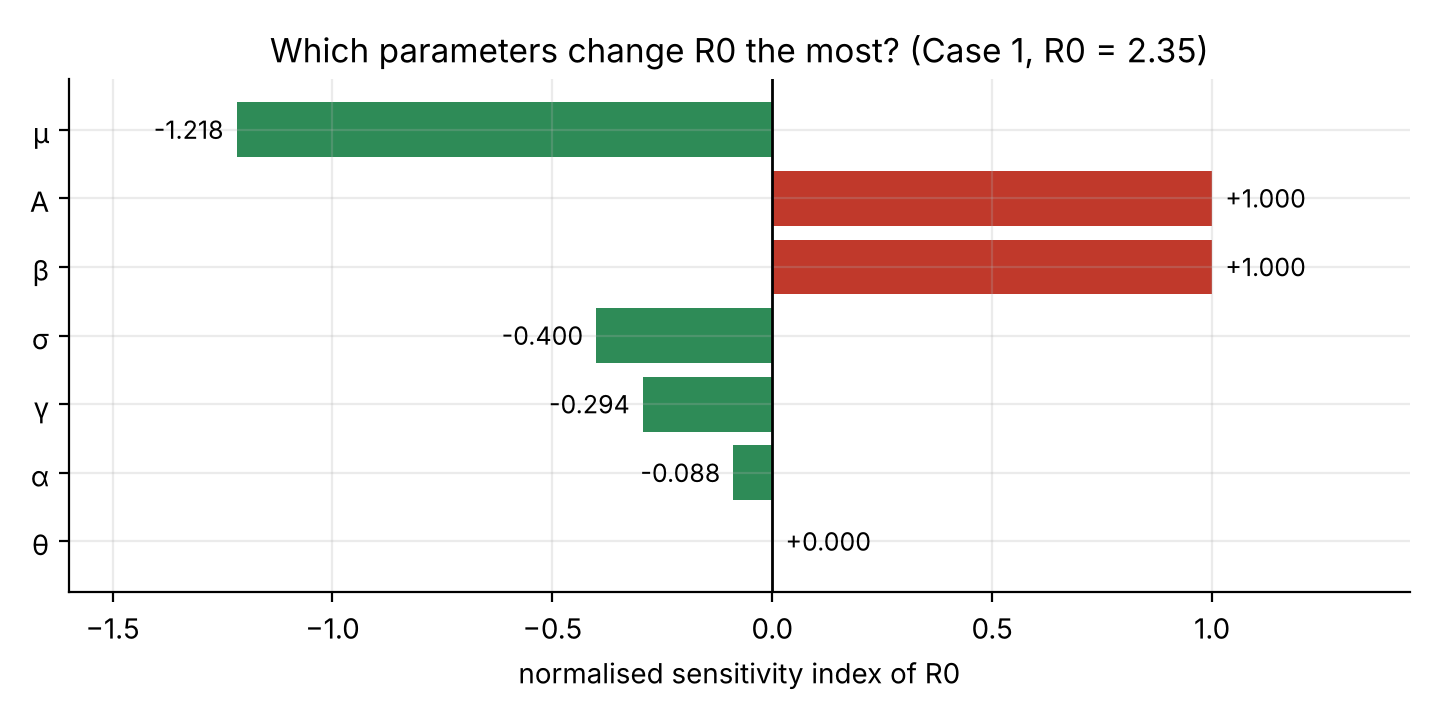
\includegraphics[width=0.9\linewidth]{charts/Fig18_Sensitivity_Indices.png}
\caption{Normalised sensitivity indices of $R_{0}$ for Case 1 (red bars raise $R_{0}$, green bars lower it).}
\end{figure}

\textbf{Explanation. }The bars show how strongly each parameter moves $R_{0}$. The longest bar is $\mu$ (\textminus{}1.22), followed by A and $\beta$ (both +1.00), then $\sigma$ (\textminus{}0.40), $\gamma$ (\textminus{}0.29) and $\alpha$ (\textminus{}0.09). The recovery rate $\theta$ has no bar because its index is zero.


\textbf{Analysis. }Because $R_{0}$ is proportional to $\beta$, the transmission rate must fall by $1 - 1/R_{0} = 57.5\%$ for $R_{0}$ to reach 1; this is the critical value $\beta \approx 1.7 \times 10^{-5}$ found in Section 6.1. The large index of $\mu$ is a consequence of the illustrative value $\mu = 0.02$: the death rate fixes both $N^* = A/\mu$ and the length of each stage, and for a realistic small $\mu$ its index is close to \textminus{}1. A cannot be controlled and $\mu$ should not be, so the useful controls are $\beta$ and the isolation rates. Among the isolation rates, $\sigma$ is more effective than $\gamma$: increasing $\sigma$ by 10\% lowers $R_{0}$ by about 4\% (from 2.353 to 2.266), while increasing $\gamma$ by 10\% lowers it by about 3\%. The index of $\alpha$ is small and negative because a faster progression shortens the exposed stage slightly more than it increases the share of people who reach $I$. Finally, $\theta$ has index zero because isolated people do not transmit; a larger $\theta$ only reduces the number of people in isolation at a given time (Section 8). These indices are local: they describe small changes of one parameter around the Case 1 values.


\section{Lockdown Scenario}

A lockdown reduces contacts between people and therefore the transmission rate $\beta$. We model this as a step change in $\beta$: the transmission rate is $\beta$ before the lockdown start day $t_{s}$, equal to $(1 - c)\beta$ between $t_{s}$ and the end day $t_{e}$, and $\beta$ again afterwards,


\begin{equation}
\beta(t) = \begin{cases}(1-c)\beta & t_s \le t < t_e,\\ \beta & \text{otherwise}\end{cases}
\end{equation}

where $c$ is the fraction by which transmission is reduced. During the lockdown the basic reproduction number becomes $(1 - c)R_{0}$. We use the Case 1 parameters $(R_{0} = 2.353)$ and $c = 0.6$, so that $R_{0}$ during lockdown is 0.94 < 1. Five scenarios were compared over 365 days:


\begin{longtable}{>{\raggedright\arraybackslash}p{\dimexpr(\linewidth-10\tabcolsep)*3300/9026\relax}>{\centering\arraybackslash}p{\dimexpr(\linewidth-10\tabcolsep)*1250/9026\relax}>{\centering\arraybackslash}p{\dimexpr(\linewidth-10\tabcolsep)*1700/9026\relax}>{\centering\arraybackslash}p{\dimexpr(\linewidth-10\tabcolsep)*1500/9026\relax}>{\centering\arraybackslash}p{\dimexpr(\linewidth-10\tabcolsep)*1276/9026\relax}}
\hline
\rowcolor[HTML]{D9E2F3}\textbf{Scenario} & \textbf{$R_{0}$ during lockdown} & \textbf{Peak of $I$ (day)} & \textbf{New infections in 365 days} & \textbf{$I$ on day 365} \\ \hline
\endhead
No lockdown & 2.35 & 697.9 (63.5) & 21,865 & 338.5 \\ \hline
Lockdown from day 30 $(c = 0.6)$, kept & 0.94 & 145.8 (39.7) & 2,188 & 4.7 \\ \hline
Lockdown days 30–120, then lifted & 0.94, then 2.35 & 635.8 (170.2) & 17,117 & 337.4 \\ \hline
Late lockdown from day 60 $(c = 0.6)$, kept & 0.94 & 689.6 (60.8) & 5,544 & 3.0 \\ \hline
Weaker lockdown from day 30 $(c = 0.4)$, kept & 1.41 & 268.6 (76.3) & 11,277 & 173.2 \\ \hline
\end{longtable}

\textit{New infections are counted as the integral of $\beta S(E + I)$. Since births keep refilling $S$ at 100 per day, this number can exceed the population size 5000.}


\subsubsection{Chart 5.1: Infected population under different lockdowns}

\begin{figure}[H]
\centering
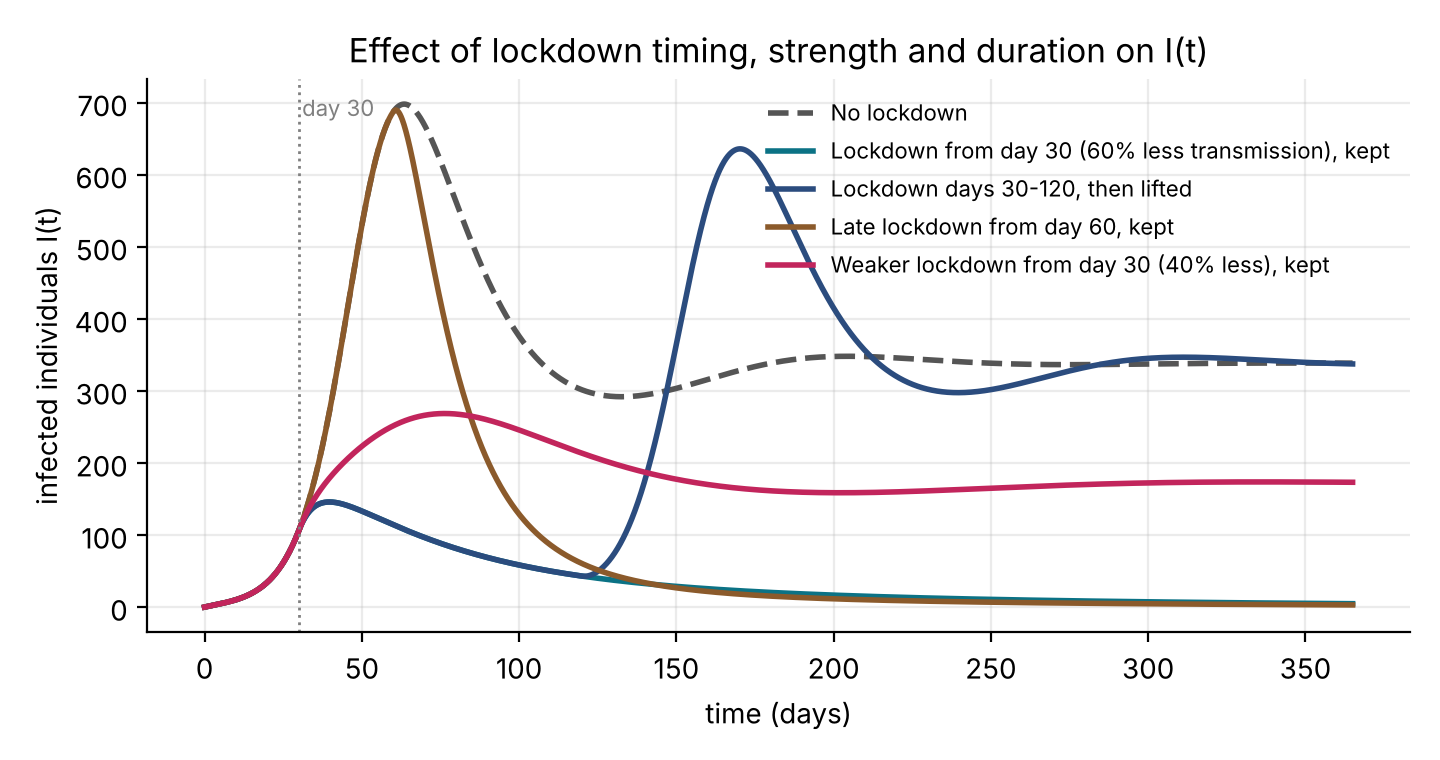
\includegraphics[width=0.9\linewidth]{charts/Fig19_Lockdown_Scenarios.png}
\caption{Infected population $I(t)$ for the five lockdown scenarios.}
\end{figure}

\textbf{Explanation. }The dashed grey curve is the no-lockdown epidemic, with its peak of 698 infected on day 63.5. With a 60\% lockdown from day 30 (teal) $I$ peaks at only 146 about ten days later and then decays to about 5 by day 365. If the same lockdown is lifted on day 120 (navy), $I$ falls to about 43 and then rises again to a second wave of 636 on day 170. A lockdown that starts late, on day 60 (brown), leaves the peak almost unchanged (690) but $I$ then falls to about 3 instead of settling near 338. A weaker lockdown with $c = 0.4$ (magenta) lowers the peak to 269 and the long-run level to about 173.


\textbf{Analysis. }The outcome depends on whether the lockdown pushes $R_{0}$ below 1. With $c = 0.6$ we have $(1 - c)R_{0} = 0.94 < 1$, so $I$ decays while the lockdown lasts. The peak still occurs about ten days after the start (day 40, not day 30), because many people are already exposed (about 220 on day 30) and move into $I$. A lockdown that is too late has little effect on the peak, since the peak is reached around day 61, but it still prevents the long endemic phase: new infections fall from 21,865 to 5,544. Lifting too early is shown by the second wave: susceptible people have not been depleted $(S$ is still about 4,500 on day 120, compared with about 2,065 without a lockdown), so when $\beta$ returns to its original value $R_{0}$ is again 2.35 and the epidemic restarts, delayed by about 107 days and almost as high (91\%) as the first peak. With $c = 0.4$ the reduced reproduction number is 1.41 > 1, so the infection is slowed but not stopped: the long-run level $I^* = [\alpha A/(k_{1}k_{2})](1 - 1/R_{0})$ falls from 338 to about 172, in agreement with the simulation. In this model a lockdown therefore works best when it is early, strong enough to give $R_{0} < 1$, and not lifted until the infection has almost disappeared.


\subsubsection{Chart 5.2: Lockdown from day 30 to day 120 and then lifted}

\begin{figure}[H]
\centering
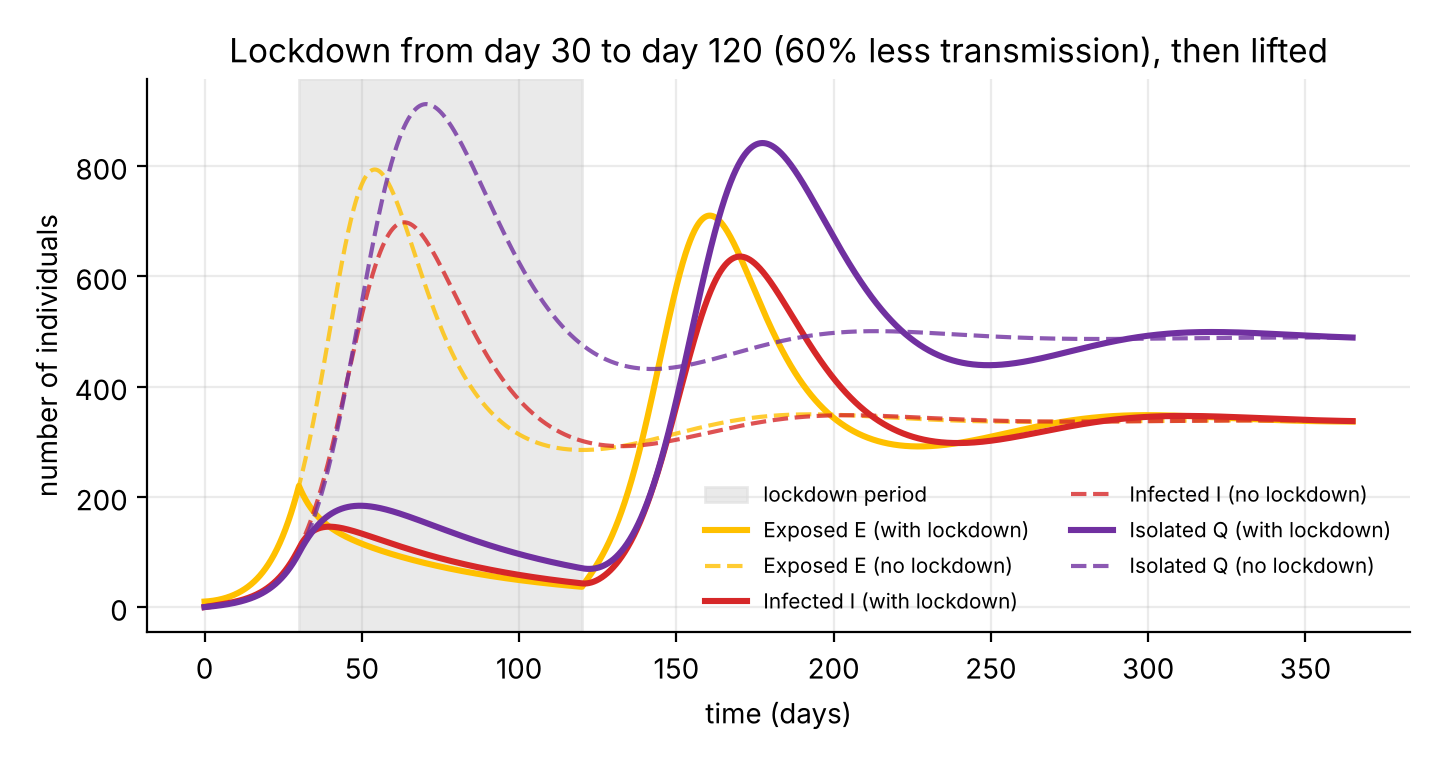
\includegraphics[width=0.9\linewidth]{charts/Fig20_Lockdown_E_I_Q.png}
\caption{$E$, $I$ and $Q$ with a lockdown from day 30 to day 120 (solid) and without lockdown (dashed). The shaded band marks the lockdown period.}
\end{figure}

\textbf{Explanation. }The solid curves (with lockdown) and the dashed curves (without lockdown) are drawn for the exposed, infected and isolated classes. During the shaded lockdown period the solid curves decrease, $E$ from about 220 to about 37 and $I$ from 146 to about 43. After the lockdown is lifted they rise again, $E$ to 710 on day 161, $I$ to 636 on day 170 and $Q$ to 842 on day 177.


\textbf{Analysis. }While $\beta$ is reduced, $dE/dt = \beta (1 -$ c)S(E $+ I) - k_{1}E$ is negative because $(1 - c)R_{0} < 1$, so $E$ falls first and $I$ and $Q$ follow in the usual order. At day 120, $S$ is still about 4,500 (the epidemic was suppressed, not allowed to run its course), so the moment $\beta$ returns to its original value the exposed class grows again. The second wave is lower than the first peak of $Q$ (842 against 912) but occurs much later, which gives time for preparation. After about day 250 the solution settles at the same endemic equilibrium $C^*$ as the no-lockdown case, because the parameters are the same: a temporary lockdown delays and flattens the epidemic but does not change the long-run state. In the Excel workbook the start day, end day and reduction $c$ can be changed (Parameters sheet) and the dashboard updates.


Limitation: real lockdowns start and end gradually and have social and economic costs which this simple model does not include.


\section{Simulation with Parameters from the Literature}

To check that the model behaves sensibly with realistic values, it was run with a parameter set based on the sources in Section 6.2. The population is taken as $N^* = 10^{6}$ (only the fractions matter) and the initial state is 10 exposed people.


\begin{longtable}{>{\raggedright\arraybackslash}p{\dimexpr(\linewidth-6\tabcolsep)*1900/9026\relax}>{\centering\arraybackslash}p{\dimexpr(\linewidth-6\tabcolsep)*2500/9026\relax}>{\raggedright\arraybackslash}p{\dimexpr(\linewidth-6\tabcolsep)*4626/9026\relax}}
\hline
\rowcolor[HTML]{D9E2F3}\textbf{Parameter} & \textbf{Value} & \textbf{Basis} \\ \hline
\endhead
$\mu$ & $3.9 \times 10^{-5}$ per day & 1/(70.7 years $\times$ 365) \cite{r13} \\ \hline
A & 38.8 per day & $A = \mu N^*$ for $N^* = 10^{6}$ \\ \hline
$\alpha$ & 0.192 per day & 1/5.2 days, incubation period \cite{r10} \\ \hline
$\sigma$ & 0.172 per day & 1/5.8 days, onset to medical contact \cite{r10} \\ \hline
$\theta$ & 0.0714 per day & 1/14 days, recovery of mild cases \cite{r12} \\ \hline
$\gamma$ & 0.05 per day & assumed (no direct estimate) \\ \hline
$\beta$ & $2.52 \times 10^{-7}$ & chosen so that $R_{0} = 2.2$ \cite{r10} \\ \hline
\end{longtable}

\subsubsection{Chart 6.1: Exposed, infected and isolated with literature-based parameters}

\begin{figure}[H]
\centering
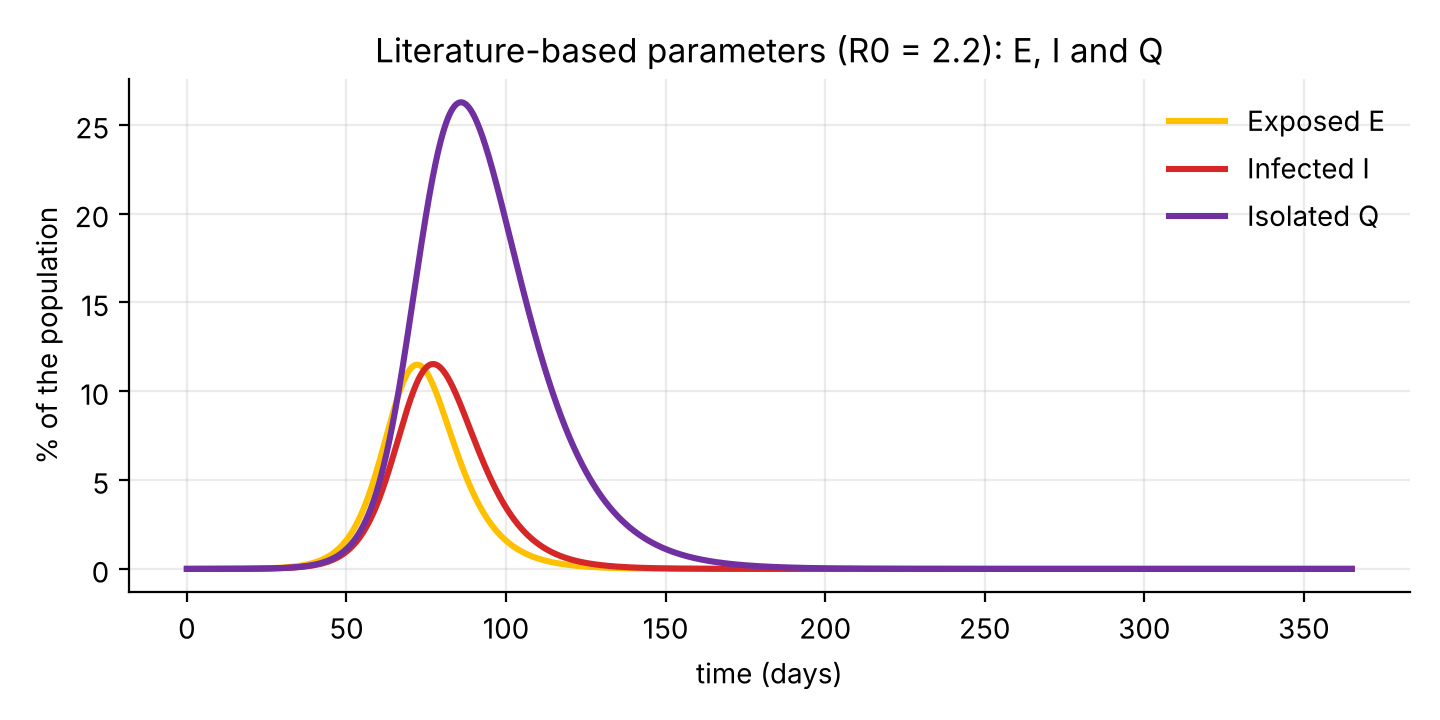
\includegraphics[width=0.9\linewidth]{charts/Fig21_Literature_Based_E_I_Q.png}
\caption{$E$, $I$ and $Q$ as percentages of the population $(R_{0} = 2.2$, literature-based parameters).}
\end{figure}

\textbf{Explanation. }All three classes rise to a single peak and then fall almost to zero within a year. The exposed class peaks at about 11.5\% of the population on day 72, the infected class at about 11.5\% on day 77, and the isolated class at about 26.3\% on day 86. By day 365 the infected fraction is practically zero.


\textbf{Analysis. }With $R_{0} = 2.2$ and no lockdown the model gives a single large wave in which the susceptible fraction falls from 100\% to a minimum of about 15.8\%, so more than 80\% of the population is infected at some time. The peak of $I$ comes later than in Case 1 (day 77 instead of day 64), partly because the epidemic starts from 10 cases in a population of one million instead of 5,000 and therefore needs more time to grow. The isolated class is the largest because people stay isolated for about two weeks $(1/\theta = 14$ days) and are fed from both $E$ and $I$. Since the realistic birth and death rates are tiny (about $4 \times 10^{-5}$ per day), susceptible people are replaced very slowly, so the approach to the endemic state described by Theorem 2 takes many years and is not visible within one year. This run shows the same qualitative behaviour as Cases 1 and 2, while its numbers come from published estimates and not from illustrative choices. It is still not a forecast: the parameters are early-epidemic estimates for China, mixing is homogeneous and no interventions are included.


\section{Extended Model: Disease Death and Vaccination}

The base model ignores deaths caused by the disease and has no vaccination. Both are added in this section, and their effect on $R_{0}$ and on the epidemic is compared with the base model.


\subsection{The extended model}

A vaccinated compartment $V$ and a disease death rate $d$ are added, with these assumptions: (1) susceptible people are vaccinated at rate $\nu$; (2) the vaccine is “leaky”: vaccinated people can still be infected, but the transmission term is multiplied by $(1 - \varepsilon )$, where $\varepsilon$ is the vaccine efficacy $(0 \le \varepsilon \le 1)$; (3) protection does not wane during the study period; (4) infected $(I)$ and isolated $(Q)$ people die of the disease at rate $d$, in addition to natural death, while exposed people do not; (5) all other assumptions of Section 2.1 hold. Deaths from the disease are counted in a variable $D$. The equations are


\begin{equation}
\frac{dS}{dt} = A-(\mu+\nu)S-\beta S(E+I)
\end{equation}

\begin{equation}
\frac{dV}{dt} = \nu S-\mu V-(1-\varepsilon)\beta V(E+I)
\end{equation}

\begin{equation}
\frac{dE}{dt} = \beta\left[S+(1-\varepsilon)V\right](E+I)-k_1E
\end{equation}

\begin{equation}
\frac{dI}{dt} = \alpha E-k_2I
\end{equation}

\begin{equation}
\frac{dQ}{dt} = \gamma E+\sigma I-k_3Q
\end{equation}

\begin{equation}
\frac{dR}{dt}=\theta Q-\mu R,\qquad \frac{dD}{dt}=d\,(I+Q)
\end{equation}

with $k_{1} = \alpha + \mu + \gamma$, $k_{2} = \sigma + \mu + d$ and $k_{3} = \theta + \mu + d$. For $\nu = 0$ and $d = 0$ the system reduces to the original model. Because deaths are removed from the population, the total $N = S + V + E + I + Q + R$ is no longer constant: $dN/dt = A - \mu N -$ d(I $+ Q)$.


\subsection{Reproduction number and threshold}

Without infection the equations for $S$ and $V$ give the disease-free equilibrium


\begin{equation}
S_0 = \frac{A}{\mu+\nu},\qquad V_0 = \frac{\nu A}{\mu(\mu+\nu)},\qquad S_0+V_0 = \frac{A}{\mu} = N^*
\end{equation}

Let $p = V_{0}/N^* = \nu /(\mu + \nu )$ be the fraction of the disease-free population that is vaccinated. New infections in the infected compartments $(E$, $I)$ occur at rate $\beta [S_{0} + (1 - \varepsilon )V_{0}] = \beta N^*(1 - \varepsilon p)$, so the next-generation matrix of Section 6 holds with $\beta N^*$ replaced by $\beta N^*(1 - \varepsilon p)$. The reproduction number with vaccination is


\begin{equation}
R_v = R_0^{(d)}(1-\varepsilon p),\qquad R_0^{(d)} = \frac{\beta N^*(k_2+\alpha)}{k_1k_2},\qquad k_2 = \sigma+\mu+d
\end{equation}

\begin{theorem}
The disease-free equilibrium of the extended model is locally asymptotically stable if $R_{v} < 1$ and unstable if $R_{v} > 1$.
\end{theorem}

\begin{proof}
At the disease-free equilibrium the Jacobian is block-triangular, as in Section 7. Its eigenvalues are $-(\mu + \nu )$, $-\mu$, $-k_{3}$ and $-\mu$, which are negative, and the two eigenvalues of the infection block with entries $\beta S_{eff} - k_{1}$, $\beta S_{eff}$, $\alpha$ and $-k_{2}$, where $S_{eff} = N^*(1 - \varepsilon p)$. The determinant of this block is $k_{1}k_{2}(1 - R_{v})$ and the argument of Theorem 1 applies with $\beta S_{eff}$ in place of $\beta N^*$: if $R_{v} < 1$ then both Routh–Hurwitz conditions hold, and if $R_{v} > 1$ the determinant is negative and there is a positive eigenvalue.
\end{proof}

Effect of the death rate. The disease death rate enters only through $k_{2}$: dying people leave the infectious class sooner, so the infectious period $1/k_{2}$ is shorter and $R_{0}$ is lower. For the Case 1 parameters:


\begin{longtable}{>{\raggedright\arraybackslash}p{\dimexpr(\linewidth-8\tabcolsep)*2200/9026\relax}>{\centering\arraybackslash}p{\dimexpr(\linewidth-8\tabcolsep)*2200/9026\relax}>{\centering\arraybackslash}p{\dimexpr(\linewidth-8\tabcolsep)*2200/9026\relax}>{\centering\arraybackslash}p{\dimexpr(\linewidth-8\tabcolsep)*2426/9026\relax}}
\hline
\rowcolor[HTML]{D9E2F3}\textbf{Death rate $d$ (per day)} & \textbf{$k_{2} = \sigma + \mu + d$} & \textbf{$R_{0}^{(d)}$} & \textbf{Change from $d = 0$} \\ \hline
\endhead
0 & 0.100 & 2.353 & – \\ \hline
0.005 & 0.105 & 2.297 & \textminus{}2.4\% \\ \hline
0.01 & 0.110 & 2.246 & \textminus{}4.5\% \\ \hline
0.02 & 0.120 & 2.157 & \textminus{}8.3\% \\ \hline
0.05 & 0.150 & 1.961 & \textminus{}16.7\% \\ \hline
\end{longtable}

\textit{Death is of course not a method of control; the table only shows that it changes $R_{0}$ through the length of the infectious period.}


Vaccination threshold. $R_{v} < 1$ is equivalent to a vaccinated share above the critical value, and the corresponding vaccination rate is


\begin{equation}
p_c = \frac{1-1/R_0^{(d)}}{\varepsilon},\qquad \nu_c = \frac{\mu\,(R_0^{(d)}-1)}{\varepsilon R_0^{(d)}-(R_0^{(d)}-1)}
\end{equation}

These exist only if $\varepsilon > 1 - 1/R_{0}^{(d)}$; if the vaccine is less effective than this, no vaccination rate can bring $R_{v}$ below 1. For $d = 0.01 (R_{0}^{(d)} = 2.246)$ and $\varepsilon = 0.9$ we get $p_{c} = 61.6\%$ and $\nu _{c} = 0.032$ per day. The formula for $p_{c}$ is the classical herd-immunity threshold, divided by the efficacy $\varepsilon$. Since new susceptible people are born at rate $\mu$, a coverage $p$ is only kept if vaccination continues at rate $\nu = p\mu /(1 - p)$.


\subsection{Simulation}

Four scenarios were simulated over 365 days with the Case 1 parameters, $\varepsilon = 0.9$, $S(0) = 4990$, $E(0) = 10$, and all other classes zero. The value $d = 0.01$ per day is deliberately large so that its effect is visible; real disease death rates are much smaller. “Long-run $I$” is the infected number after 4,000 days, when the solution has settled.


\begin{longtable}{>{\raggedright\arraybackslash}p{\dimexpr(\linewidth-12\tabcolsep)*3000/9037\relax}>{\centering\arraybackslash}p{\dimexpr(\linewidth-12\tabcolsep)*1100/9037\relax}>{\centering\arraybackslash}p{\dimexpr(\linewidth-12\tabcolsep)*1700/9037\relax}>{\centering\arraybackslash}p{\dimexpr(\linewidth-12\tabcolsep)*1100/9037\relax}>{\centering\arraybackslash}p{\dimexpr(\linewidth-12\tabcolsep)*1100/9037\relax}>{\centering\arraybackslash}p{\dimexpr(\linewidth-12\tabcolsep)*1037/9037\relax}}
\hline
\rowcolor[HTML]{D9E2F3}\textbf{Scenario} & \textbf{$R_{0}$ or $R_{v}$} & \textbf{Peak of $I$ (day)} & \textbf{$I$ on day 365} & \textbf{Deaths in 365 days} & \textbf{Long-run $I$} \\ \hline
\endhead
No death, no vaccination & 2.35 & 697.9 (63.5) & 338.5 & 0 & 338.2 \\ \hline
Disease death $d = 0.01$ & 2.25 & 624.6 (63.6) & 297.0 & 2,522 & 296.7 \\ \hline
$d = 0.01$, $\nu = 0.02$ (50\% vaccinated) & 1.24 & 140.0 (98.9) & 109.5 & 894 & 109.7 \\ \hline
$d = 0.01$, $\nu = 0.06$ (75\% vaccinated) & 0.73 & 12.3 (27.0) & 0.0 & 19 & 0 \\ \hline
\end{longtable}

\subsubsection{Chart 7.1: Infected population with disease death and vaccination}

\begin{figure}[H]
\centering
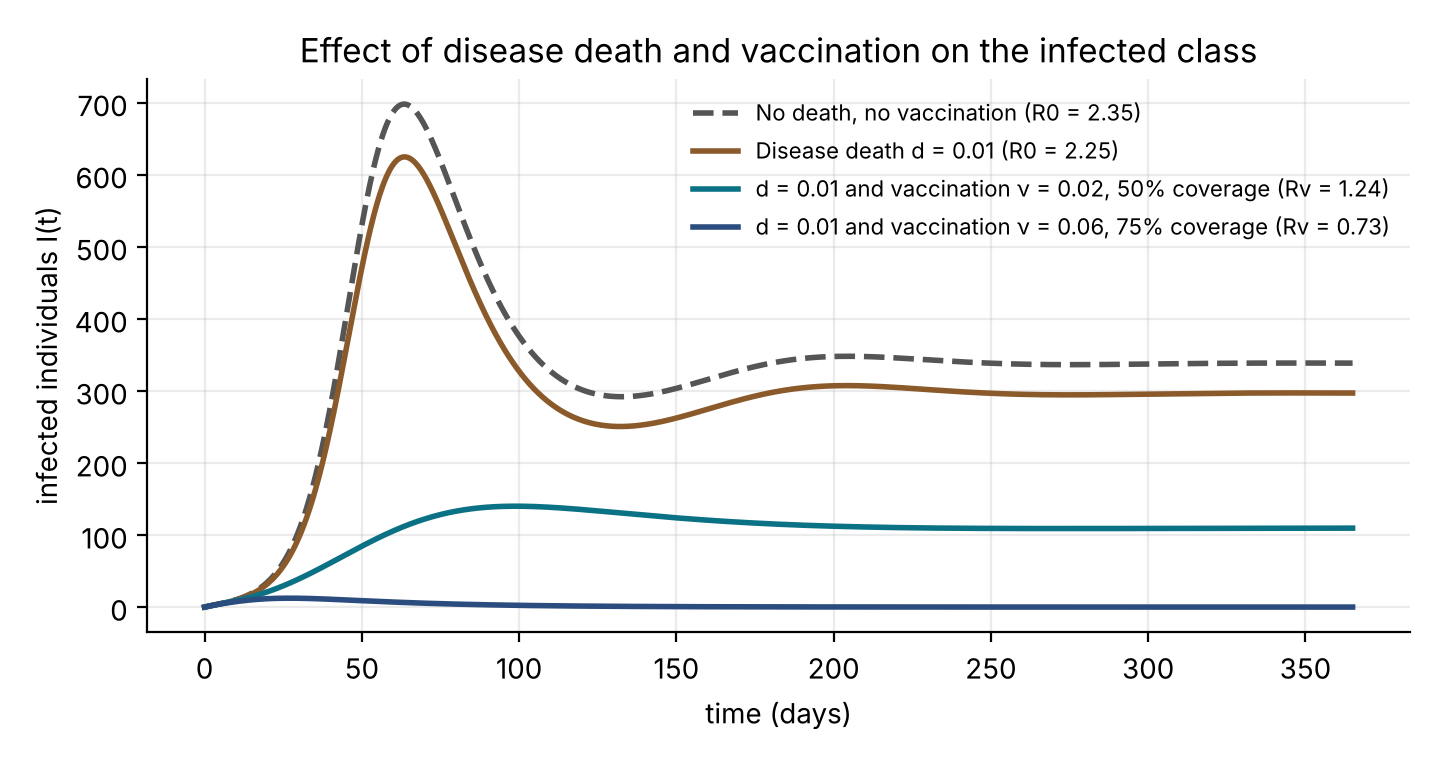
\includegraphics[width=0.9\linewidth]{charts/Fig22_Extended_Model_Infected.png}
\caption{Infected population $I(t)$ for the four scenarios of the extended model.}
\end{figure}

\textbf{Explanation. }The dashed grey curve is the base epidemic with a peak of 698 infected. With a disease death rate $d = 0.01$ (brown) the peak falls to 625 and the long-run level to 297. With vaccination at $\nu = 0.02$ (teal) the peak is only 140 and is delayed to day 99, and $I$ then settles near 110. With $\nu = 0.06$ (navy) there is no epidemic: $I$ stays below 13 and is zero by day 365.


\textbf{Analysis. }Death removes people from $I$ and $Q$, which shortens the infectious period and lowers $R_{0}$ from 2.35 to 2.25; the peak falls by about 10\%, but at the cost of 2,522 deaths in one year. Vaccination moves susceptible people to $V$, where they are infected ten times less easily $(\varepsilon = 0.9)$. With $\nu = 0.02$ the vaccinated share is $p = \nu /(\mu + \nu ) = 50\%$, so $R_{v} = 2.246 \times (1 - 0.9 \times 0.5) = 1.24$. This is still above 1, so the infection is slowed and reduced but persists, at a long-run level of 110 against 297 without vaccination, and deaths fall to 894. With $\nu = 0.06$ the vaccinated share is 75\%, above the critical value 61.6\%, so $R_{v} = 0.73 < 1$ and, as Theorem 3 predicts, the infection dies out. The small bump of 12 infected people comes from the 10 initially exposed individuals and is not an epidemic wave (compare Case 2, Section 10.2).


\subsubsection{Chart 7.2: Reproduction number against vaccination coverage}

\begin{figure}[H]
\centering
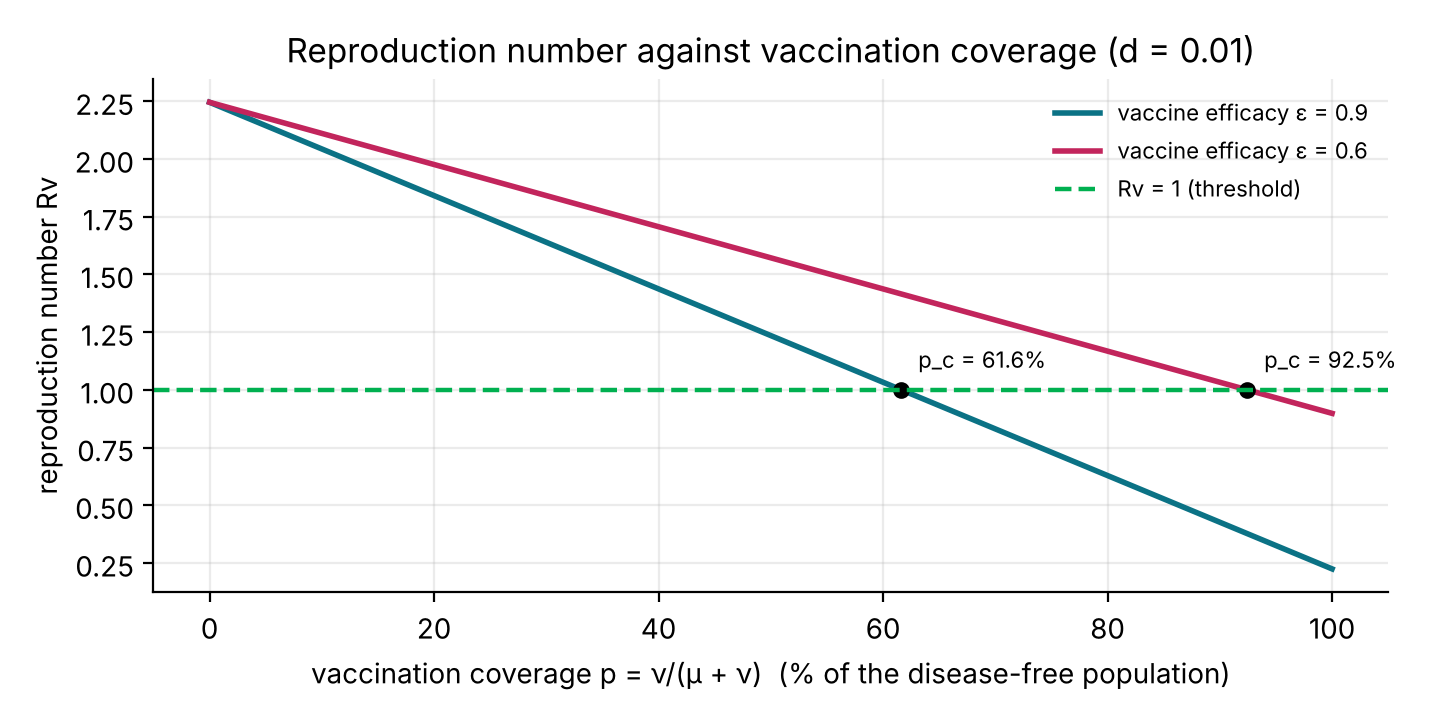
\includegraphics[width=0.9\linewidth]{charts/Fig23_Rv_vs_Coverage.png}
\caption{$R_{v}$ as a function of the vaccinated share $p$, for two vaccine efficacies $(d = 0.01)$.}
\end{figure}

\textbf{Explanation. }Both lines start at $R_{0}^{(d)} = 2.25$ when nobody is vaccinated and fall in a straight line as coverage increases. The teal line $(\varepsilon = 0.9)$ crosses the threshold $R_{v} = 1$ at a coverage of 61.6\%. The pink line $(\varepsilon = 0.6)$ crosses it only at 92.5\%.


\textbf{Analysis. }The straight lines follow from $R_{v} = R_{0}^{(d)}(1 - \varepsilon p)$, whose slope is $-\varepsilon R_{0}^{(d)}$. A vaccine of lower efficacy needs a much higher coverage to reach the same effect: $p_{c} = (1 - 1/R_{0}^{(d)})/\varepsilon$ rises from 61.6\% to 92.5\% when $\varepsilon$ falls from 0.9 to 0.6. If $\varepsilon$ were at most $1 - 1/R_{0}^{(d)} = 0.555$, even 100\% coverage would not push $R_{v}$ below 1. In this model, therefore, vaccine efficacy and coverage matter equally; the product $\varepsilon p$ is what reduces $R_{0}$.


Limitation of the extended model: the vaccine does not wane, recovered and exposed people are not vaccinated, and there are no age groups or priority groups.


\section{Numerical Check: Euler's Method against Runge–Kutta 4}

The Excel workbook uses Euler's method, which is simple but only first-order accurate. This section measures its error and compares it with the fourth-order Runge–Kutta method (RK4).


\subsection{The two methods}

For the system dy/dt = f(y) with step $h$, Euler's method is


\begin{equation}
y_{n+1} = y_n + h\,f(y_n)
\end{equation}

and RK4 uses four slopes per step,


\begin{equation}
k_1 = f(y_n),\quad k_2 = f\!\left(y_n+\tfrac{h k_1}{2}\right),\quad k_3 = f\!\left(y_n+\tfrac{h k_2}{2}\right),\quad k_4 = f(y_n+h k_3)
\end{equation}

\begin{equation}
y_{n+1} = y_n + \frac{h}{6}\left(k_1+2k_2+2k_3+k_4\right)
\end{equation}

The error of Euler's method accumulated over a fixed time is proportional to $h$ (first order); that of RK4 is proportional to $h^{4}$ (fourth order). RK4 needs four evaluations of f per step, Euler only one.


\subsection{Results}

Both methods were applied to Case 1 over 360 days and compared with a reference solution computed with an adaptive eighth-order Dormand–Prince method at tolerance $10^{-13}$. The error is the largest difference $|I_{h}(t) - I_{ref}(t)|$ at the grid times; the peak of $I$ is 697.9 people.


\begin{longtable}{>{\raggedright\arraybackslash}p{\dimexpr(\linewidth-12\tabcolsep)*1100/9026\relax}>{\centering\arraybackslash}p{\dimexpr(\linewidth-12\tabcolsep)*1100/9026\relax}>{\centering\arraybackslash}p{\dimexpr(\linewidth-12\tabcolsep)*1700/9026\relax}>{\centering\arraybackslash}p{\dimexpr(\linewidth-12\tabcolsep)*1500/9026\relax}>{\centering\arraybackslash}p{\dimexpr(\linewidth-12\tabcolsep)*1700/9026\relax}>{\centering\arraybackslash}p{\dimexpr(\linewidth-12\tabcolsep)*1926/9026\relax}}
\hline
\rowcolor[HTML]{D9E2F3}\textbf{$h$ (days)} & \textbf{Steps} & \textbf{Euler error in $I$ (people)} & \textbf{Euler error (\% of peak)} & \textbf{RK4 error in $I$ (people)} & \textbf{RK4 error (\% of peak)} \\ \hline
\endhead
5 & 72 & 234.9 & 33.7\% & 0.316 & $4.5 \times 10^{-2}\%$ \\ \hline
2 & 180 & 99.0 & 14.2\% & $1.2 \times 10^{-2}$ & $1.8 \times 10^{-3}\%$ \\ \hline
1 & 360 & 50.1 & 7.18\% & $8.7 \times 10^{-4}$ & $1.3 \times 10^{-4}\%$ \\ \hline
0.5 & 720 & 25.1 & 3.59\% & $5.8 \times 10^{-5}$ & $8.3 \times 10^{-6}\%$ \\ \hline
0.2 & 1800 & 10.0 & 1.44\% & $1.5 \times 10^{-6}$ & $2.2 \times 10^{-7}\%$ \\ \hline
0.1 & 3600 & 5.021 & 0.72\% & $9.7 \times 10^{-8}$ & $1.4 \times 10^{-8}\%$ \\ \hline
0.05 & 7200 & 2.511 & 0.36\% & $6.2 \times 10^{-9}$ & $8.8 \times 10^{-10}\%$ \\ \hline
0.01 & 36000 & 0.502 & $7.2 \times 10^{-2}\%$ & $8.0 \times 10^{-10}$ & $1.1 \times 10^{-10}\%$ \\ \hline
\end{longtable}

\textit{The row $h = 0.1$ is the step used in the Excel workbook. The RK4 error at $h = 0.01$ is limited by rounding errors and by the accuracy of the reference solution.}


\subsubsection{Chart 8.1: Error against step size}

\begin{figure}[H]
\centering
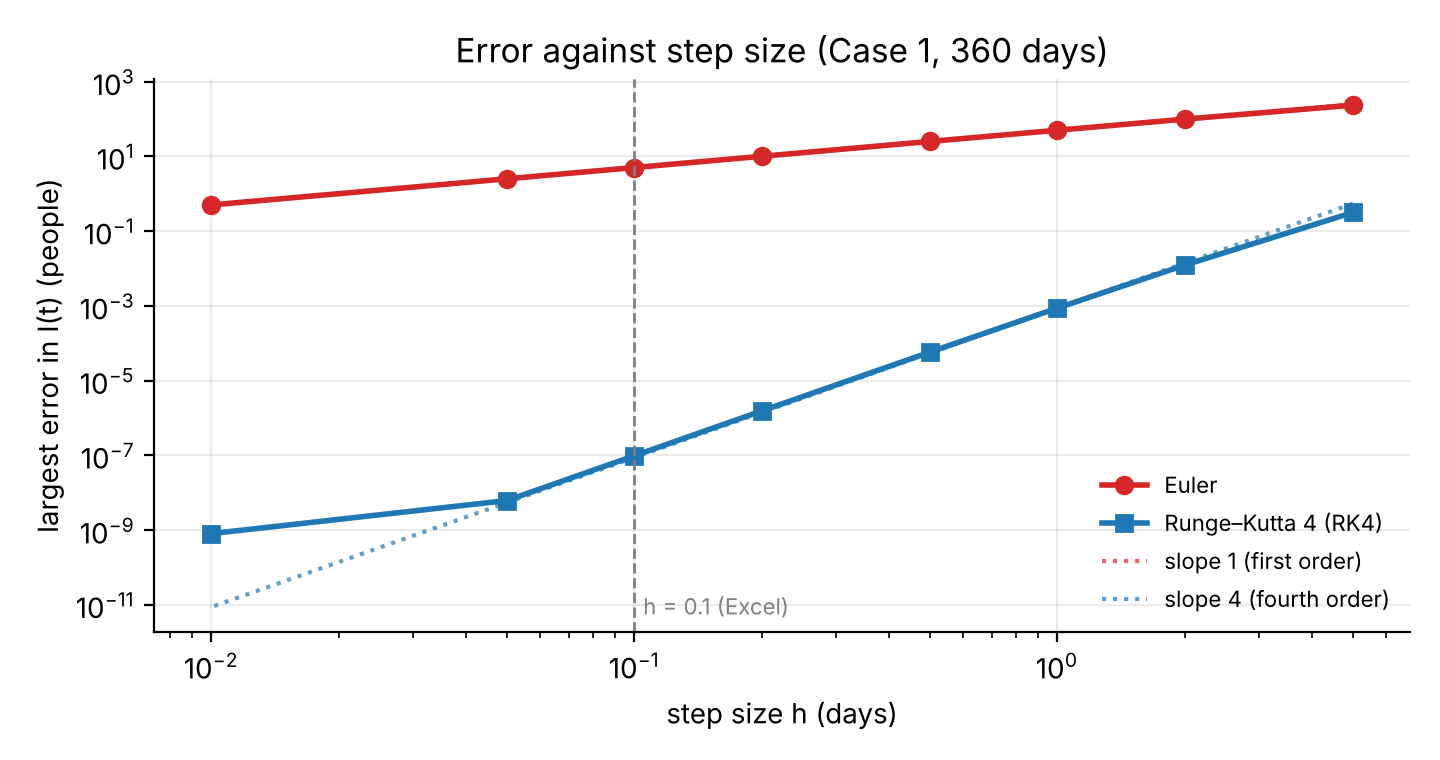
\includegraphics[width=0.9\linewidth]{charts/Fig24_Euler_vs_RK4_Error.png}
\caption{Largest error in $I(t)$ against step size $h$ for Euler's method and RK4 (logarithmic axes).}
\end{figure}

\textbf{Explanation. }Both axes are logarithmic. The red Euler line rises with a slope of about 1: halving $h$ from 0.1 to 0.05 halves the error from 5.0 to 2.5 people. The blue RK4 line is much lower and much steeper, with a slope of about 4 (measured 3.93 between $h = 0.1$ and $h = 2)$: halving $h$ reduces its error by roughly a factor of 16. The vertical dashed line marks the step 0.1 used in the Excel workbook.


\textbf{Analysis. }The slopes confirm the orders of the methods. RK4 is far more efficient even though each step costs four evaluations: with $h = 1$ (360 steps, 1,440 evaluations) its error is under 0.001 people, whereas Euler with $h = 0.01$ (36,000 evaluations) still has an error of 0.5 people. For the Excel charts the Euler error at $h = 0.1$ is at most about 5 people, which is 0.7\% of the peak (Euler gives a peak of 699.6 against the true 697.9); this is invisible in a chart but should not be quoted as an exact value. With $h = 0.1$ the RK4 error is about $10^{-7}$ people.


\subsubsection{Chart 8.2: A very coarse step}

\begin{figure}[H]
\centering
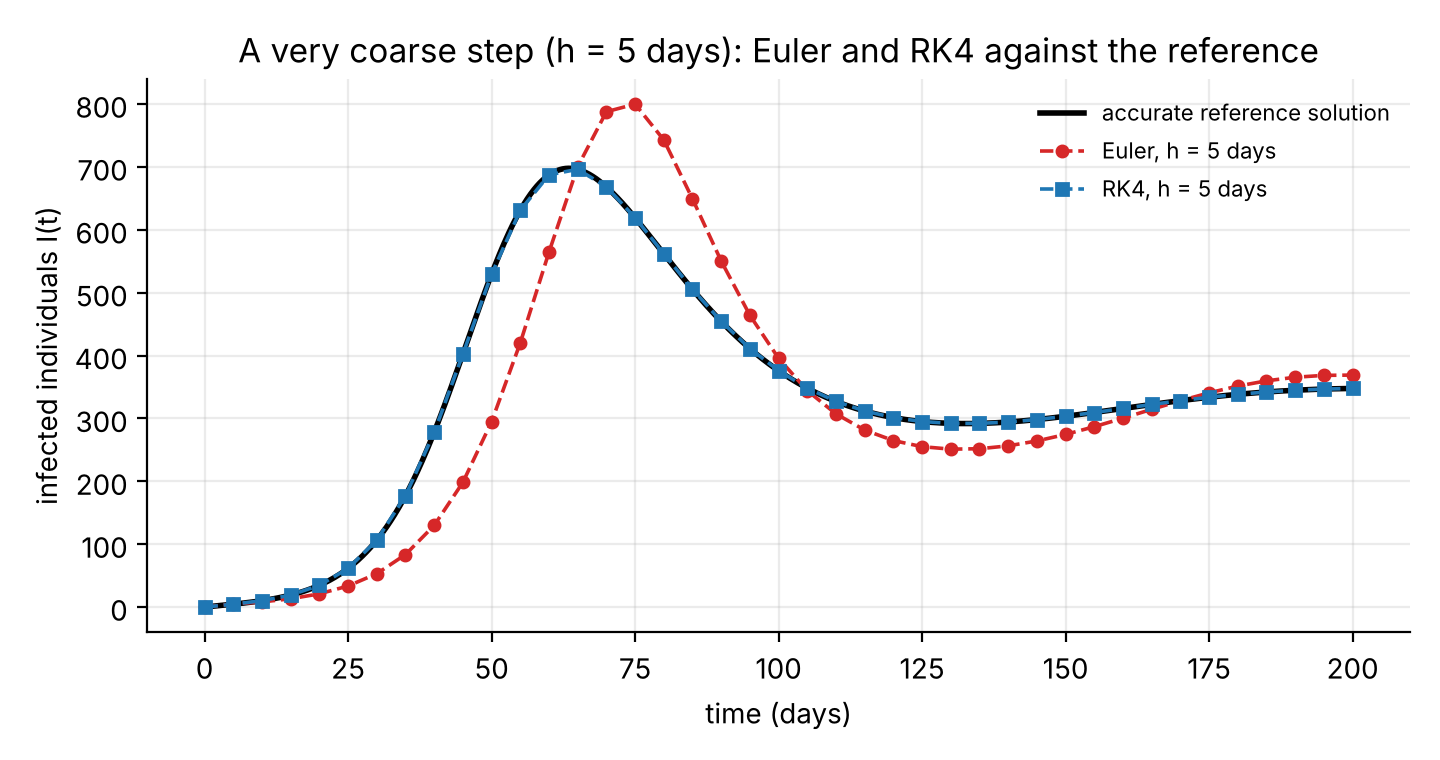
\includegraphics[width=0.9\linewidth]{charts/Fig25_Coarse_Step_Comparison.png}
\caption{Infected population $I(t)$ computed with step $h = 5$ days by Euler's method and RK4, against the accurate solution.}
\end{figure}

\textbf{Explanation. }The black curve is the accurate solution. The blue RK4 points with a step of five days lie almost exactly on it. The red Euler points are visibly wrong: the epidemic wave is delayed by about 10 days and its peak is 800 instead of 698.


\textbf{Analysis. }Euler's method advances each step with the slope at the start of the interval. When the curve is bending, as near the peak, this overshoots and delays the wave. RK4 averages four slopes taken inside the interval, so it follows the curve even with a coarse step. This is why the step size for Euler's method has to be small, and why RK4 is preferred when accuracy is needed. A C++ program with RK4 is given in Appendix $E$.


\subsection{Conclusion}

Euler's method with $h = 0.1$ is accurate enough for the charts in the Excel workbook (error below 1\% of the peak). When exact values are needed, or when a larger step is used, RK4 should be used. The figures in this report were computed with an accurate adaptive solver and agree with RK4.


\section{Why There Is No Closed-Form Solution}

Some parts of the system can be solved by integrating factors. For example, multiplying $dR/dt + \mu R = \theta Q$ by $e^{\mu t}$ gives


\begin{equation}
R(t) = e^{-\mu t}\left[R(0)+\int_0^t \theta Q(s)\,e^{\mu s}\,ds\right]
\end{equation}

and similarly for $Q$ and $I$:


\begin{equation}
Q(t) = e^{-k_3 t}\left[Q(0)+\int_0^t (\gamma E+\sigma I)\,e^{k_3 s}\,ds\right]
\end{equation}

\begin{equation}
I(t) = e^{-k_2 t}\left[I(0)+\int_0^t \alpha E(s)\,e^{k_2 s}\,ds\right]
\end{equation}

However, these formulas contain the other unknown functions $E(s)$ and $I(s)$ inside the integrals. The equations for $S$ and $E$ contain the product $\beta S(E + I)$ of two unknown functions, so the system is nonlinear and coupled and cannot be separated. By contrast, a linear equation dx/dt = ax has the solution $x_{0}e^{at}$, but here the coefficient of $I$ in $dI/dt = \alpha E - k_{2}I$ depends on $E$, which depends on $S$, which changes with time. Hence explicit formulas for $S(t)$, $E(t)$, $I(t)$ are not available. We therefore rely on equilibrium analysis, $R_{0}$, stability theory and numerical simulation, as in Sections 6–10.


\section{Findings, Limitations, Recommendations and Conclusion}

\subsection{Findings}

\begin{itemize}
\item $R_{0} = (\beta A/\mu )[1/k_{1} + \alpha /(k_{1}k_{2})]$ is a threshold parameter. For $R_{0} < 1$ the disease-free equilibrium is locally asymptotically stable; for $R_{0} > 1$ it is unstable and a unique, locally asymptotically stable endemic equilibrium exists.
\item The equilibria exchange stability at $R_{0} = 1$ (a forward transcritical bifurcation); there is no endemic state below the threshold.
\item In the example with $R_{0} = 2.35$ the outbreak peaks around day 64 with about 698 infected, then oscillates and settles at the endemic level of 338 infected.
\item Raising $\gamma$ or $\sigma$ always lowers $R_{0}$. Because exposed people transmit, isolating infected people alone may not be enough; isolation of exposed people $(\gamma )$ is needed.
\item The recovery rate $\theta$ does not enter $R_{0}$. A larger $\theta$ reduces the number of people isolated at any time $(Q^*$ and $R^*)$ but not the transmission.
\item Closed-form solutions are not available because of the nonlinear term $\beta S(E + I)$.
\item $R_{0}$ is proportional to $\beta$ and A. Among the isolation parameters $\sigma$ (index \textminus{}0.40) is more influential than $\gamma$ (\textminus{}0.29), and $\theta$ has no effect on $R_{0}$.
\item A lockdown that brings $R_{0}$ below 1 suppresses the epidemic, but only if it is early and not lifted too soon: in the example lifting it on day 120 produced a second wave almost as high as the first peak.
\item With parameters taken from the literature $(R_{0} = 2.2)$ the model shows one large epidemic wave, with the same qualitative behaviour as the illustrative cases.
\item In the extended model the disease death rate shortens the infectious period and lowers $R_{0}$ slightly (from 2.35 to 2.25 for $d = 0.01)$. With vaccination $R_{v} = R_{0}(1 - \varepsilon p)$, so the infection dies out when the vaccinated share exceeds $(1 - 1/R_{0})/\varepsilon$, which is 61.6\% for $\varepsilon = 0.9$.
\item Euler's method is first-order and RK4 is fourth-order accurate. With the step 0.1 day of the Excel workbook the Euler error in $I(t)$ is at most about 5 people (0.7\% of the peak), while the RK4 error is about $10^{-7}$.
\end{itemize}

\subsection{Limitations}

\begin{itemize}
\item Parameter values are illustrative and were not fitted to real data.
\item The incidence $\beta S(E + I)$ depends on the population size; the standard incidence $\beta S(E +$ I)/N makes $R_{0}$ independent of population size.
\item Isolation is assumed perfect, immunity is assumed permanent (reinfection occurs in reality), and all parameters are constant (lockdowns and behaviour change are not represented).
\item The stability results are local.
\item The lockdown is a simple step change in $\beta$; real measures change gradually and have costs not modelled here.
\end{itemize}

\subsection{Recommendations (within the model)}

\begin{itemize}
\item Reduce the transmission rate $\beta$ (masks, distancing, reduced contacts) so that $R_{0}$ falls below 1.
\item Increase the isolation rates $\gamma$ and $\sigma$ through rapid testing, contact tracing and quarantine, with special attention to exposed contacts.
\item Use $R_{0} < 1$ as the target: starting from a small number of cases, the infection then dies out in the model.
\item Improve treatment and care to raise $\theta$, which lowers the load of people in isolation or care at any time.
\item Start control measures early and keep them in place until $R_{0}$ has been brought below 1 for long enough; lifting them too soon allows a second wave.
\end{itemize}

\subsection{Possible extensions}

\begin{itemize}
\item compare standard (frequency-dependent) and mass-action incidence;
\item use smooth or data-driven changes of $\beta (t)$ instead of a sudden step;
\item let vaccine protection wane, vaccinate exposed or recovered people, and add age groups;
\item use stochastic versions of the model for small outbreaks; and
\item fit the model to data for individual states, such as West Bengal, with a reporting fraction.
\end{itemize}

\subsection{Conclusion}

A deterministic SEIQR model with demography was formulated and analysed. The basic reproduction number $R_{0}$ governs its behaviour: below 1 the infection dies out, above 1 an epidemic occurs followed by a stable endemic level. Faster isolation of both exposed and infected individuals reduces $R_{0}$ and the size of the outbreak, and in the example doubling the isolation rates reduces the epidemic peak by about 80\%. Mathematical modelling therefore provides a useful framework for understanding and controlling infectious diseases such as COVID-19.


\addcontentsline{toc}{section}{References}
\begin{thebibliography}{99}
\bibitem{r1} Kermack, W. O. and McKendrick, A. G. (1927). A contribution to the mathematical theory of epidemics. Proceedings of the Royal Society A, 115(772), 700–721.
\bibitem{r2} Bairagi, N. Introductory Mathematical Biology. U. N. Dhur \& Sons Pvt. Ltd., Kolkata.
\bibitem{r3} Hethcote, H. W. (2000). The mathematics of infectious diseases. SIAM Review, 42(4), 599–653.
\bibitem{r4} Murray, J. D. (2002). Mathematical Biology I: An Introduction, 3rd edition. Springer.
\bibitem{r5} van den Driessche, P. and Watmough, J. (2002). Reproduction numbers and sub-threshold endemic equilibria for compartmental models of disease transmission. Mathematical Biosciences, 180, 29–48.
\bibitem{r6} Diekmann, O., Heesterbeek, J. A. P. and Roberts, M. G. (2010). The construction of next-generation matrices for compartmental epidemic models. Journal of the Royal Society Interface, 7(47), 873–885.
\bibitem{r7} Castillo-Chavez, C. and Song, B. (2004). Dynamical models of tuberculosis and their applications. Mathematical Biosciences and Engineering, 1(2), 361–404.
\bibitem{r8} World Health Organization. Coronavirus disease (COVID-19) pandemic: situation reports and dashboard. \url{https://www.who.int}
\bibitem{r9} Lauer, S. A. et al. (2020). The incubation period of coronavirus disease 2019 (COVID-19) from publicly reported confirmed cases: estimation and application. Annals of Internal Medicine, 172(9), 577–582.
\bibitem{r10} Li, Q. et al. (2020). Early transmission dynamics in Wuhan, China, of novel coronavirus–infected pneumonia. New England Journal of Medicine, 382(13), 1199–1207.
\bibitem{r11} He, X. et al. (2020). Temporal dynamics in viral shedding and transmissibility of COVID-19. Nature Medicine, 26(5), 672–675 (author correction: Nature Medicine, 26, 1491–1493).
\bibitem{r12} World Health Organization (2020). Report of the WHO-China Joint Mission on Coronavirus Disease 2019 (COVID-19), 16–24 February 2020. WHO, Geneva.
\bibitem{r13} World Bank. World Development Indicators: India, life expectancy at birth and crude birth rate (retrieved through FRED, Federal Reserve Bank of St. Louis).
\bibitem{r14} Chitnis, N., Hyman, J. M. and Cushing, J. M. (2008). Determining important parameters in the spread of malaria through the sensitivity analysis of a mathematical model. Bulletin of Mathematical Biology, 70, 1272–1296.
\end{thebibliography}

\clearpage
\appendix

\section{Excel simulation workbook}

File name: SEIQR\_COVID19\_Simulation.xlsx. The workbook solves the SEIQR equations day by day with Euler's method, using only spreadsheet formulas, and draws the charts automatically. Only the blue cells on the Parameters sheet need to be changed.


\textbf{Link: }\textit{[paste the shared link to the Excel workbook here]}


\begin{longtable}{>{\raggedright\arraybackslash}p{\dimexpr(\linewidth-4\tabcolsep)*2300/9026\relax}>{\raggedright\arraybackslash}p{\dimexpr(\linewidth-4\tabcolsep)*6726/9026\relax}}
\hline
\rowcolor[HTML]{D9E2F3}\textbf{Sheet} & \textbf{Contents} \\ \hline
\endhead
Read\_Me & Purpose, method, colour legend and assumptions. \\ \hline
Parameters & All inputs for Case 1 and Case 2 and the lockdown inputs; published estimates with sources; $R_{0}$, equilibria and the stability conclusion calculated by formulas. \\ \hline
Sim\_R0\_gt1 & Calculation only: the day-by-day Euler table for Case 1 $(R_{0} = 2.35)$, 3,650 steps. \\ \hline
Sim\_R0\_gt1\_Graphs & Dashboard for Case 1: separate charts of $S$, $E$, $I$, $Q$, $R$ and of $E$, $I$, $Q$ together, with a summary table. \\ \hline
Sim\_R0\_lt1 & Calculation only: the day-by-day Euler table for Case 2 $(R_{0} = 0.59)$, 3,650 steps. \\ \hline
Sim\_R0\_lt1\_Graphs & Dashboard for Case 2: separate charts of $S$, $E$, $I$, $Q$, $R$ and of $E$, $I$, $Q$ together, with a summary table. \\ \hline
R0\_Sensitivity & $R_{0}$ for different isolation rates $(\gamma$, $\sigma )$ and transmission rates $(\beta )$, the critical $\beta$, and the sensitivity index of $R_{0}$ to every parameter with a chart. \\ \hline
Sim\_Lockdown & Calculation only: the model with a lockdown (transmission reduced between two chosen days) next to the no-lockdown result. \\ \hline
Sim\_Lockdown\_Graphs & Dashboard for the lockdown scenario: $S$, $E$, $I$, $Q$, $R$ with and without lockdown, the step in $\beta (t)$, and a summary table. \\ \hline
\end{longtable}

A second, separate workbook, SEIQR\_COVID19\_India\_Fit.xlsx, fits the model to real daily COVID-19 data for India (4 March 2020 to 10 January 2021). Its Read\_Me sheet describes the data source, the method and its limitations.


\textbf{Link: }\textit{[paste the shared link to the data-fit workbook here]}


\section{Charts}

All charts of this report are supplied as separate image files (PNG) with the file names below, so that they can be reused in a presentation.


\textbf{Link: }\textit{[paste the shared link to the charts folder here]}


\begin{longtable}{>{\raggedright\arraybackslash}p{\dimexpr(\linewidth-6\tabcolsep)*1200/9026\relax}>{\raggedright\arraybackslash}p{\dimexpr(\linewidth-6\tabcolsep)*5100/9026\relax}>{\raggedright\arraybackslash}p{\dimexpr(\linewidth-6\tabcolsep)*2726/9026\relax}}
\hline
\rowcolor[HTML]{D9E2F3}\textbf{Figure} & \textbf{Chart} & \textbf{File name} \\ \hline
\endhead
1 & Flow diagram of the SEIQR model & Fig01\_Flow\_Diagram.png \\ \hline
2 & Bifurcation diagram at $R_{0} = 1$ & Fig02\_Bifurcation.png \\ \hline
3 & Case 1: susceptible $S(t)$ & Fig03\_Case1\_Susceptible.png \\ \hline
4 & Case 1: exposed $E(t)$ & Fig04\_Case1\_Exposed.png \\ \hline
5 & Case 1: infected $I(t)$ & Fig05\_Case1\_Infected.png \\ \hline
6 & Case 1: isolated $Q(t)$ & Fig06\_Case1\_Isolated.png \\ \hline
7 & Case 1: recovered $R(t)$ & Fig07\_Case1\_Recovered.png \\ \hline
8 & Case 1: $E$, $I$ and $Q$ together & Fig08\_Case1\_E\_I\_Q\_together.png \\ \hline
9 & Case 2: susceptible $S(t)$ & Fig09\_Case2\_Susceptible.png \\ \hline
10 & Case 2: exposed $E(t)$ & Fig10\_Case2\_Exposed.png \\ \hline
11 & Case 2: infected $I(t)$ & Fig11\_Case2\_Infected.png \\ \hline
12 & Case 2: isolated $Q(t)$ & Fig12\_Case2\_Isolated.png \\ \hline
13 & Case 2: recovered $R(t)$ & Fig13\_Case2\_Recovered.png \\ \hline
14 & Case 2: $E$, $I$ and $Q$ together & Fig14\_Case2\_E\_I\_Q\_together.png \\ \hline
15 & S–I phase plane, Case 1 & Fig15\_PhasePlane\_Case1.png \\ \hline
16 & S–I phase plane, Case 2 & Fig16\_PhasePlane\_Case2.png \\ \hline
17 & Effect of isolation on $I(t)$ & Fig17\_Isolation\_Effect.png \\ \hline
18 & Sensitivity indices of $R_{0}$ & Fig18\_Sensitivity\_Indices.png \\ \hline
19 & Lockdown scenarios: $I(t)$ & Fig19\_Lockdown\_Scenarios.png \\ \hline
20 & Lockdown days 30–120: $E$, $I$ and $Q$ & Fig20\_Lockdown\_E\_I\_Q.png \\ \hline
21 & Literature-based parameters: $E$, $I$ and $Q$ & Fig21\_Literature\_Based\_E\_I\_Q.png \\ \hline
22 & Extended model: infected population & Fig22\_Extended\_Model\_Infected.png \\ \hline
23 & $R_{v}$ against vaccination coverage & Fig23\_Rv\_vs\_Coverage.png \\ \hline
24 & Euler against RK4: error against step size & Fig24\_Euler\_vs\_RK4\_Error.png \\ \hline
25 & Euler against RK4: coarse step & Fig25\_Coarse\_Step\_Comparison.png \\ \hline
\end{longtable}

\section{Python code used for the charts}

The following code solves the model for Case 1 and plots the five compartments. Changing beta to 1e-5 gives Case 2. It can be run free of charge on Google Colab.


\begin{lstlisting}[language=Python]
import numpy as np
import matplotlib.pyplot as plt
from scipy.integrate import solve_ivp

A, mu, beta = 100, 0.02, 4e-5
alpha, gamma, sigma, theta = 0.1, 0.05, 0.08, 0.07
k1, k2, k3 = alpha + mu + gamma, sigma + mu, theta + mu

def model(t, y):
    S, E, I, Q, R = y
    inf = beta * S * (E + I)
    return [A - mu * S - inf,
            inf - k1 * E,
            alpha * E - k2 * I,
            gamma * E + sigma * I - k3 * Q,
            theta * Q - mu * R]

t = np.linspace(0, 365, 3651)
sol = solve_ivp(model, [0, 365], [4990, 10, 0, 0, 0], t_eval=t)

for y, name in zip(sol.y, ["S", "E", "I", "Q", "R"]):
    plt.figure()
    plt.plot(t, y)
    plt.xlabel("time (days)")
    plt.ylabel(name)
plt.show()
\end{lstlisting}

\section{C++ version of the simulation}

The same model can be solved in C++ with Euler's method. The program writes the results to a CSV file, which can be opened in Excel to draw the charts. For Case 1 it gives $R_{0} = 2.353$ and a peak of 699.6 infected people on day 63.7, the same as the Excel workbook. The source file is supplied as seiqr.cpp.


\begin{lstlisting}[language=C++]
// SEIQR COVID-19 model solved with Euler's method (basic C++)
#include <iostream>
#include <fstream>
#include <cmath>
using namespace std;

int main() {
    // parameters (Case 1: R0 > 1). For Case 2 change beta to 1e-5.
    double A = 100, mu = 0.02, beta = 4e-5;
    double alpha = 0.1, gamma = 0.05, sigma = 0.08, theta = 0.07;
    double k1 = alpha + mu + gamma, k2 = sigma + mu, k3 = theta + mu;

    // basic reproduction number
    double N = A / mu;
    double R0 = beta * N * (1.0 / k1 + alpha / (k1 * k2));
    cout << "R0 = " << R0 << endl;

    // initial values and step size
    double S = 4990, E = 10, I = 0, Q = 0, R = 0;
    double h = 0.1, T = 365;
    int steps = (int)(T / h);

    ofstream out("seiqr_output.csv");
    out << "t,S,E,I,Q,R\n";
    double peakI = 0, dayPeak = 0;

    for (int n = 0; n <= steps; n++) {
        double t = n * h;
        out << t << "," << S << "," << E << "," << I << "," << Q << "," << R << "\n";
        if (I > peakI) { peakI = I; dayPeak = t; }

        // rates of change
        double inf = beta * S * (E + I);
        double dS = A - mu * S - inf;
        double dE = inf - k1 * E;
        double dI = alpha * E - k2 * I;
        double dQ = gamma * E + sigma * I - k3 * Q;
        double dR = theta * Q - mu * R;

        // Euler update
        S += h * dS; E += h * dE; I += h * dI; Q += h * dQ; R += h * dR;
    }
    cout << "Peak infected = " << peakI << " on day " << dayPeak << endl;
    out.close();
    return 0;
}

\end{lstlisting}

\section{C++ version with RK4}

The same model solved with the fourth-order Runge–Kutta method. For Case 1 it gives a peak of 697.875 infected people on day 63.5, which agrees with the accurate solution (Section 16). The source file is supplied as seiqr\_rk4.cpp.


\begin{lstlisting}[language=C++]
// SEIQR COVID-19 model solved with the fourth-order Runge-Kutta method (RK4)
#include <iostream>
#include <fstream>
using namespace std;

// parameters (Case 1: R0 > 1). For Case 2 change beta to 1e-5.
const double A = 100, mu = 0.02, beta = 4e-5;
const double alpha = 0.1, gamma_ = 0.05, sigma = 0.08, theta = 0.07;
const double k1 = alpha + mu + gamma_, k2 = sigma + mu, k3 = theta + mu;

// right-hand side of the five equations: dy/dt = f(y)
void f(const double y[5], double dy[5]) {
    double S = y[0], E = y[1], I = y[2], Q = y[3], R = y[4];
    double inf = beta * S * (E + I);
    dy[0] = A - mu * S - inf;
    dy[1] = inf - k1 * E;
    dy[2] = alpha * E - k2 * I;
    dy[3] = gamma_ * E + sigma * I - k3 * Q;
    dy[4] = theta * Q - mu * R;
}

int main() {
    double N = A / mu;
    double R0 = beta * N * (1.0 / k1 + alpha / (k1 * k2));
    cout << "R0 = " << R0 << endl;

    double y[5] = {4990, 10, 0, 0, 0};
    double h = 0.1, T = 365;
    int steps = (int)(T / h + 0.5);

    ofstream out("seiqr_rk4_output.csv");
    out << "t,S,E,I,Q,R\n";
    double peakI = 0, dayPeak = 0;

    for (int n = 0; n <= steps; n++) {
        double t = n * h;
        out << t << "," << y[0] << "," << y[1] << "," << y[2] << "," << y[3] << "," << y[4] << "\n";
        if (y[2] > peakI) { peakI = y[2]; dayPeak = t; }

        // one RK4 step: four slopes a, b, c, d
        double a[5], b[5], c[5], d[5], tmp[5];
        f(y, a);
        for (int i = 0; i < 5; i++) tmp[i] = y[i] + 0.5 * h * a[i];
        f(tmp, b);
        for (int i = 0; i < 5; i++) tmp[i] = y[i] + 0.5 * h * b[i];
        f(tmp, c);
        for (int i = 0; i < 5; i++) tmp[i] = y[i] + h * c[i];
        f(tmp, d);
        for (int i = 0; i < 5; i++) y[i] += h / 6.0 * (a[i] + 2 * b[i] + 2 * c[i] + d[i]);
    }
    cout << "Peak infected = " << peakI << " on day " << dayPeak << endl;
    out.close();
    return 0;
}

\end{lstlisting}

\section{Scilab versions of the simulations}

Scilab is free software, similar to MATLAB, which can solve the model with its built-in ode command and draw the charts. The five scripts below solve the same equations as the Python and C++ programs. The charts from the first two scripts were compared with Figures 3 to 7 and 9 to 13 of this report, and the peaks and minima agree (for example, $I$ peaks at about 698 on day 63.5 in Case 1). To run a script, open it in Scilab (File, then Open) and click Run. The source files are supplied as .sce files.


\subsubsection{F.1 seiqr\_charts.sce: Case 1, compartments $S$, $E$, $I$, $Q$, $R$}

Solves the model for Case 1 $(R_{0} = 2.35)$ and draws five separate charts. It reproduces Figures 3 to 7 and prints the peak of $I$ (about 698 on day 63.5).


\begin{lstlisting}[language=Matlab]
// SEIQR COVID-19 model: the five compartments (Case 1: beta = 4e-5; Case 2: beta = 1e-5)
// Run in Scilab: File > Open, then click Run.
A = 100; mu = 0.02; beta = 4e-5;
alpha = 0.1; gamma = 0.05; sigma = 0.08; theta = 0.07;
k1 = alpha + mu + gamma; k2 = sigma + mu; k3 = theta + mu;

function dy = seiqr(t, y)
    S = y(1); E = y(2); I = y(3); Q = y(4); R = y(5);
    inf = beta * S * (E + I);
    dy = [A - mu*S - inf;
          inf - k1*E;
          alpha*E - k2*I;
          gamma*E + sigma*I - k3*Q;
          theta*Q - mu*R];
endfunction

t = 0:0.1:365;
y0 = [4990; 10; 0; 0; 0];
y = ode(y0, 0, t, seiqr);

names = ["S" "E" "I" "Q" "R"];
for i = 1:5
    scf(i);
    plot(t, y(i,:));
    xlabel("time (days)");
    ylabel(names(i));
end
[pk, ip] = max(y(3,:));
mprintf("Peak of I = %.1f on day %.1f\n", pk, t(ip));   // Case 1: about 698 on day 63.5
\end{lstlisting}

\subsubsection{F.2 seiqr\_charts\_Case2.sce: Case 2, compartments $S$, $E$, $I$, $Q$, $R$}

The same script with $\beta = 1 \times 10^{-5} (R_{0} = 0.59)$. It reproduces Figures 9 to 13 and prints the peak of $I$ (about 3.6 on day 10.8).


\begin{lstlisting}[language=Matlab]
// SEIQR COVID-19 model: the five compartments, Case 2 (R0 = 0.59, beta = 1e-5)
// Run in Scilab: File > Open, then click Run.
A = 100; mu = 0.02; beta = 1e-5;
alpha = 0.1; gamma = 0.05; sigma = 0.08; theta = 0.07;
k1 = alpha + mu + gamma; k2 = sigma + mu; k3 = theta + mu;

function dy = seiqr(t, y)
    S = y(1); E = y(2); I = y(3); Q = y(4); R = y(5);
    inf = beta * S * (E + I);
    dy = [A - mu*S - inf;
          inf - k1*E;
          alpha*E - k2*I;
          gamma*E + sigma*I - k3*Q;
          theta*Q - mu*R];
endfunction

t = 0:0.1:365;
y0 = [4990; 10; 0; 0; 0];
y = ode(y0, 0, t, seiqr);

names = ["S" "E" "I" "Q" "R"];
for i = 1:5
    scf(i);
    plot(t, y(i,:));
    xlabel("time (days)");
    ylabel(names(i));
end
[pk, ip] = max(y(3,:));
mprintf("Peak of I = %.1f on day %.1f\n", pk, t(ip));   // Case 2: about 3.6 on day 10.8
\end{lstlisting}

\subsubsection{F.3 seiqr\_phase\_plane.sce: S–I phase plane}

Plots $S$ against $I$ from five starting points. With casenr = 1 it reproduces Figure 15 $(R_{0} > 1)$; with casenr = 2 it reproduces Figure 16 $(R_{0} < 1)$.


\begin{lstlisting}[language=Matlab]
// SEIQR phase plane: S against I from five different starting points
// casenr = 1: R0 = 2.35 (curves spiral into the endemic point); casenr = 2: R0 = 0.59 (curves go to the disease-free point)
casenr = 1;
A = 100; mu = 0.02;
alpha = 0.1; gamma = 0.05; sigma = 0.08; theta = 0.07;
k1 = alpha + mu + gamma; k2 = sigma + mu; k3 = theta + mu;
if casenr == 1 then
    beta = 4e-5; T = 500; Sstar = 2125; Istar = 338.2;      // endemic point C*
else
    beta = 1e-5; T = 150; Sstar = 5000; Istar = 0;          // disease-free point C0
end

function dy = seiqr(t, y)
    S = y(1); E = y(2); I = y(3); Q = y(4); R = y(5);
    inf = beta * S * (E + I);
    dy = [A - mu*S - inf;
          inf - k1*E;
          alpha*E - k2*I;
          gamma*E + sigma*I - k3*Q;
          theta*Q - mu*R];
endfunction

t = 0:0.1:T;
starts = [4990 4900 3000 1000 4000;      // S(0)
            10  100  300   50   20;      // E(0)
             0    0    0    0    0;
             0    0    0    0    0;
             0    0    0    0    0];
clf();
for j = 1:5
    y = ode(starts(:,j), 0, t, seiqr);
    plot(y(1,:), y(3,:));
    plot(y(1,1), y(3,1), "ko");              // black dot = starting point
end
plot(Sstar, Istar, "r*");                    // red star = equilibrium point
xlabel("S (susceptible)");
ylabel("I (infected)");
\end{lstlisting}

\subsubsection{F.4 seiqr\_lockdown.sce: lockdown scenarios}

Plots the infected population for the five lockdown scenarios of Section 13 and prints the peak of each (Figure 19). The lockdown start day, end day and reduction are set in the vectors ts\_, te\_ and c\_.


\begin{lstlisting}[language=Matlab]
// SEIQR lockdown scenarios (Case 1 parameters): infected population I(t)
// beta is cut by the fraction c between day ts and day te.
global bb
A = 100; mu = 0.02; beta = 4e-5;
alpha = 0.1; gamma = 0.05; sigma = 0.08; theta = 0.07;
k1 = alpha + mu + gamma; k2 = sigma + mu; k3 = theta + mu;

function dy = seiqrL(t, y)
    global bb
    S = y(1); E = y(2); I = y(3); Q = y(4); R = y(5);
    inf = bb * S * (E + I);
    dy = [A - mu*S - inf;
          inf - k1*E;
          alpha*E - k2*I;
          gamma*E + sigma*I - k3*Q;
          theta*Q - mu*R];
endfunction

dt = 0.1;
y0 = [4990; 10; 0; 0; 0];
//          no lockdown | day 30 kept | 30-120 lifted | day 60 kept | weaker (40%)
c_  = [0      0.6    0.6    0.6    0.4];
ts_ = [30     30     30     60     30];
te_ = [120    365    120    365    365];
cols = ["k" "c" "b" "m" "r"];

clf();
for s = 1:5
    c = c_(s); ts = ts_(s); te = te_(s);
    bb = beta;
    tA = dt:dt:ts;
    yA = ode(y0, 0, tA, seiqrL);
    tt = [0 tA]; yy = [y0 yA];
    bb = beta*(1 - c);
    if te > ts then
        tB = ts+dt:dt:te;
        yB = ode(yy(:,$), ts, tB, seiqrL);
        tt = [tt tB]; yy = [yy yB];
    end
    bb = beta;
    if te < 365 then
        tC = te+dt:dt:365;
        yC = ode(yy(:,$), te, tC, seiqrL);
        tt = [tt tC]; yy = [yy yC];
    end
    plot(tt, yy(3,:), cols(s));
    [pk, ip] = max(yy(3,:));
    mprintf("scenario %d: peak I = %.1f on day %.1f\n", s, pk, tt(ip));
end
xlabel("time (days)"); ylabel("infected I(t)");
legend("No lockdown", "Lockdown from day 30, kept", "Lockdown days 30-120, then lifted", "Late lockdown from day 60, kept", "Weaker lockdown from day 30 (40%)");
// expected peaks: 698 (day 63.5), 146 (day 40), 636 (day 170), 690 (day 61), 269 (day 76)
\end{lstlisting}

\subsubsection{F.5 seiqr\_euler\_vs\_rk4.sce: Euler against RK4}

Part 1 prints and plots the largest error in $I(t)$ for several step sizes (Figure 24); Part 2 compares Euler and RK4 with the very coarse step of 5 days (Figure 25).


\begin{lstlisting}[language=Matlab]
// Euler's method against RK4 for the SEIQR model (Case 1)
// Part 1: largest error in I(t) for different step sizes.  Part 2: a very coarse step (h = 5 days).
A = 100; mu = 0.02; beta = 4e-5;
alpha = 0.1; gamma = 0.05; sigma = 0.08; theta = 0.07;
k1 = alpha + mu + gamma; k2 = sigma + mu; k3 = theta + mu;

function dy = seiqr(t, y)
    S = y(1); E = y(2); I = y(3); Q = y(4); R = y(5);
    inf = beta * S * (E + I);
    dy = [A - mu*S - inf;
          inf - k1*E;
          alpha*E - k2*I;
          gamma*E + sigma*I - k3*Q;
          theta*Q - mu*R];
endfunction

y0 = [4990; 10; 0; 0; 0];

// ---- Part 1: error against step size (360 days) ----
T = 360;
hs = [5 2 1 0.5 0.2 0.1 0.05 0.01];
errE = []; errK = [];
for h = hs
    n = round(T/h);
    t = (0:n)*h;
    yref = [y0, ode(y0, 0, t(2:$), 1e-12, 1e-12, seiqr)];   // accurate reference solution
    ye = zeros(5, n+1); yk = zeros(5, n+1);
    ye(:,1) = y0; yk(:,1) = y0;
    for i = 1:n
        y = ye(:,i);
        ye(:,i+1) = y + h*seiqr(0, y);                       // Euler step
        y = yk(:,i);
        s1 = seiqr(0, y);
        s2 = seiqr(0, y + h/2*s1);
        s3 = seiqr(0, y + h/2*s2);
        s4 = seiqr(0, y + h*s3);
        yk(:,i+1) = y + h/6*(s1 + 2*s2 + 2*s3 + s4);         // RK4 step
    end
    errE = [errE, max(abs(ye(3,:) - yref(3,:)))];
    errK = [errK, max(abs(yk(3,:) - yref(3,:)))];
    mprintf("h = %g: Euler error %g, RK4 error %g\n", h, errE($), errK($));
end
scf(1); clf();
plot2d("ll", hs', [errE' errK'], [5 2]);
xlabel("step size h (days)"); ylabel("largest error in I(t) (people)");
legend("Euler", "RK4");
// expected at h = 0.1: Euler about 5.0, RK4 about 1e-7

// ---- Part 2: a very coarse step, h = 5 days ----
h = 5; T = 200; n = T/h; t = (0:n)*h;
ye = zeros(5, n+1); yk = zeros(5, n+1);
ye(:,1) = y0; yk(:,1) = y0;
for i = 1:n
    y = ye(:,i);
    ye(:,i+1) = y + h*seiqr(0, y);
    y = yk(:,i);
    s1 = seiqr(0, y);
    s2 = seiqr(0, y + h/2*s1);
    s3 = seiqr(0, y + h/2*s2);
    s4 = seiqr(0, y + h*s3);
    yk(:,i+1) = y + h/6*(s1 + 2*s2 + 2*s3 + s4);
end
tf = 0:0.5:T;
yf = [y0, ode(y0, 0, tf(2:$), 1e-12, 1e-12, seiqr)];
scf(2); clf();
plot(tf, yf(3,:), "k");
plot(t, ye(3,:), "r-o");
plot(t, yk(3,:), "b-s");
xlabel("time (days)"); ylabel("infected I(t)");
legend("accurate solution", "Euler, h = 5", "RK4, h = 5");
// expected peaks: Euler about 800, RK4 about 696, accurate solution about 698
\end{lstlisting}

\end{document}
